\documentclass[../../main/main.tex]{subfiles}
\graphicspath{{./figures/}}

\dominitoc
\faketableofcontents

\makeatletter
\renewcommand{\@chapapp}{\'Electrocin\'etique -- chapitre}
\makeatother

% \toggletrue{student}
% \HideSolutionstrue
\toggletrue{corrige}
\renewcommand{\mycol}{black}
% \renewcommand{\mycol}{gray}

\begin{document}
\setcounter{chapter}{6}

\chapter{Filtrage lin\'eaire}

\vfill

\begin{prgm}
	\begin{tcb}*(ror)"know"{Savoirs}
		\begin{itemize}[label=$\diamond$, leftmargin=10pt]
			\item Analyser la décomposition fournie d'un signal périodique en une
			      somme de fonctions sinusoïdales.
			\item Définir la valeur moyenne et la valeur efficace d'un signal.
			\item Interpréter le fait que le carré de la valeur efficace d'un signal
			      périodique est égal à la somme des carrés des valeurs efficaces de
			      ses harmoniques.
			\item Utiliser les échelles logarithmiques et interpréter les zones
			      rectilignes des diagrammes de \textsc{Bode} en amplitude d'après
			      l'expression de la fonction de transfert.
			\item Choisir un modèle de filtre en fonction d'un cahier des charges.
			\item Détecter le caractère non linéaire d'un système par l'apparition de
			      nouvelles fréquences.
		\end{itemize}
	\end{tcb}
	\begin{tcb}*(ror)"how"{Savoir-faire}
		\begin{itemize}[label=$\diamond$, leftmargin=10pt]
			\item Établir par le calcul la valeur efficace d'un signal sinusoïdal.
			\item Tracer le diagramme de \textsc{Bode} (amplitude et phase)
			      associé à une fonction de transfert d'ordre~1.
			\item Utiliser une fonction de transfert donnée d'ordre 1 ou 2 (ou ses
			      représentations graphiques) pour étudier la réponse d'un système
			      linéaire à une excitation sinusoïdale, à une somme finie
			      d'excitations sinusoïdales, à un signal périodique.
			\item Expliciter les conditions d'utilisation d'un filtre en tant que
			      moyenneur, intégrateur, ou dérivateur.
			\item Expliquer l'intérêt, pour garantir leur fonctionnement lors de mises
			      en cascade, de réaliser des filtres de tension de faible impédance
			      de sortie et forte impédance d'entrée.
			\item Expliquer la nature du filtrage introduit par un dispositif
			      mécanique (sismomètre, amortisseur, accéléromètre, etc.).
		\end{itemize}
	\end{tcb}
\end{prgm}

\vfill

\newpage

\vspace*{\fill}
\minitoc
\vspace*{\fill}

À travers les précédents chapitres, nous avons mis en place des moyens d'étudier
l'amplitude d'un signal de sortie (tension $u_C$, élongation $x$) en fonction de
la pulsation d'un signal d'entrée sinusoïdal. Dans la pratique, les signaux
purement sinusoïdaux sont rares et sont en réalité des signaux complexes,
comportant de nombreuses fréquences. La lumière blanche, par exemple, est un
signal lumineux composé d'une continuité de longueur d'ondes (allant du violet
au rouge dans le visible), qui se décompose en ses longueurs d'ondes
constitutives sous certaines conditions~: chacune de ses couleurs est déviée
différemment lors du passage dans un prise par exemple.
\bigbreak
L'objectif de ce chapitre est d'étudier des signaux complexes, qu'on décomposera
en somme de signaux sinusoïdaux, et leur traitement par des systèmes traitant
différemment ces longueurs d'ondes -- qu'on appelle des filtres. Ils sont au
cœur de toutes les innovations technologiques du \textsc{XX}\ieme\ et
\textsc{XXI}\ieme\ siècles, qui reposent entièrement sur le traitement du
signal. Cela s'applique aux transfert de données, à la création et diffusion de
musique, et même à la couleur bleue du ciel. Commençons par revenir sur les
signaux périodiques.

% https://phyanim.sciences.univ-nantes.fr/Ondes/son/analyseur.php !!

\vspace*{\fill}

\newpage

\section{Signaux périodiques}
\subsection{Période}
\begin{tcb*}(defi){Période}
	\psw{
		\[
			s(t) \quad \text{périodique}
			\Lra
			\exists T~: \forall t \in \Rb^{+}, s(t+T) = s(t)
		\]
	}
	\vspace{-15pt}
\end{tcb*}
\begin{tcb*}(appl)<lfnt>{Périodicité}
	Montrer que le signal $s(t) = A \sin(\wt)$ a une période $T =
		\frac{2\pi}{\w}$.
	\tcblower
	\psw{
		\[
			s \left( t + \frac{2\pi}{\w} \right) =
			A \left( \w \left( t + \frac{2\pi}{\w} \right) \right) =
			A \sin(\wt + 2\pi) = A \sin(\wt)
			\qed
		\]
	}
	\vspace{-15pt}
\end{tcb*}

\subsection{Moyenne}
\begin{tcb*}(defi){Valeur moyenne}
	Pour un \textbf{signal périodique} $s(t)$, on définit sa valeur moyenne
	$\moy{s(t)}$ par
	\psw{
		\[
			\moy{s(t)} = \frac{1}{T}\int _{0}^{T} s(t) \dd{t}
		\]
	}
	\vspace{-15pt}
\end{tcb*}

\begin{tcb*}[sidebyside, lefthand ratio=.4](appl){Moyenne d'un cosinus décalé}
	Calculer la valeur moyenne du signal
	\[
		s(t) = S_0 + A\cos(\wt)
	\]
	\begin{center}
		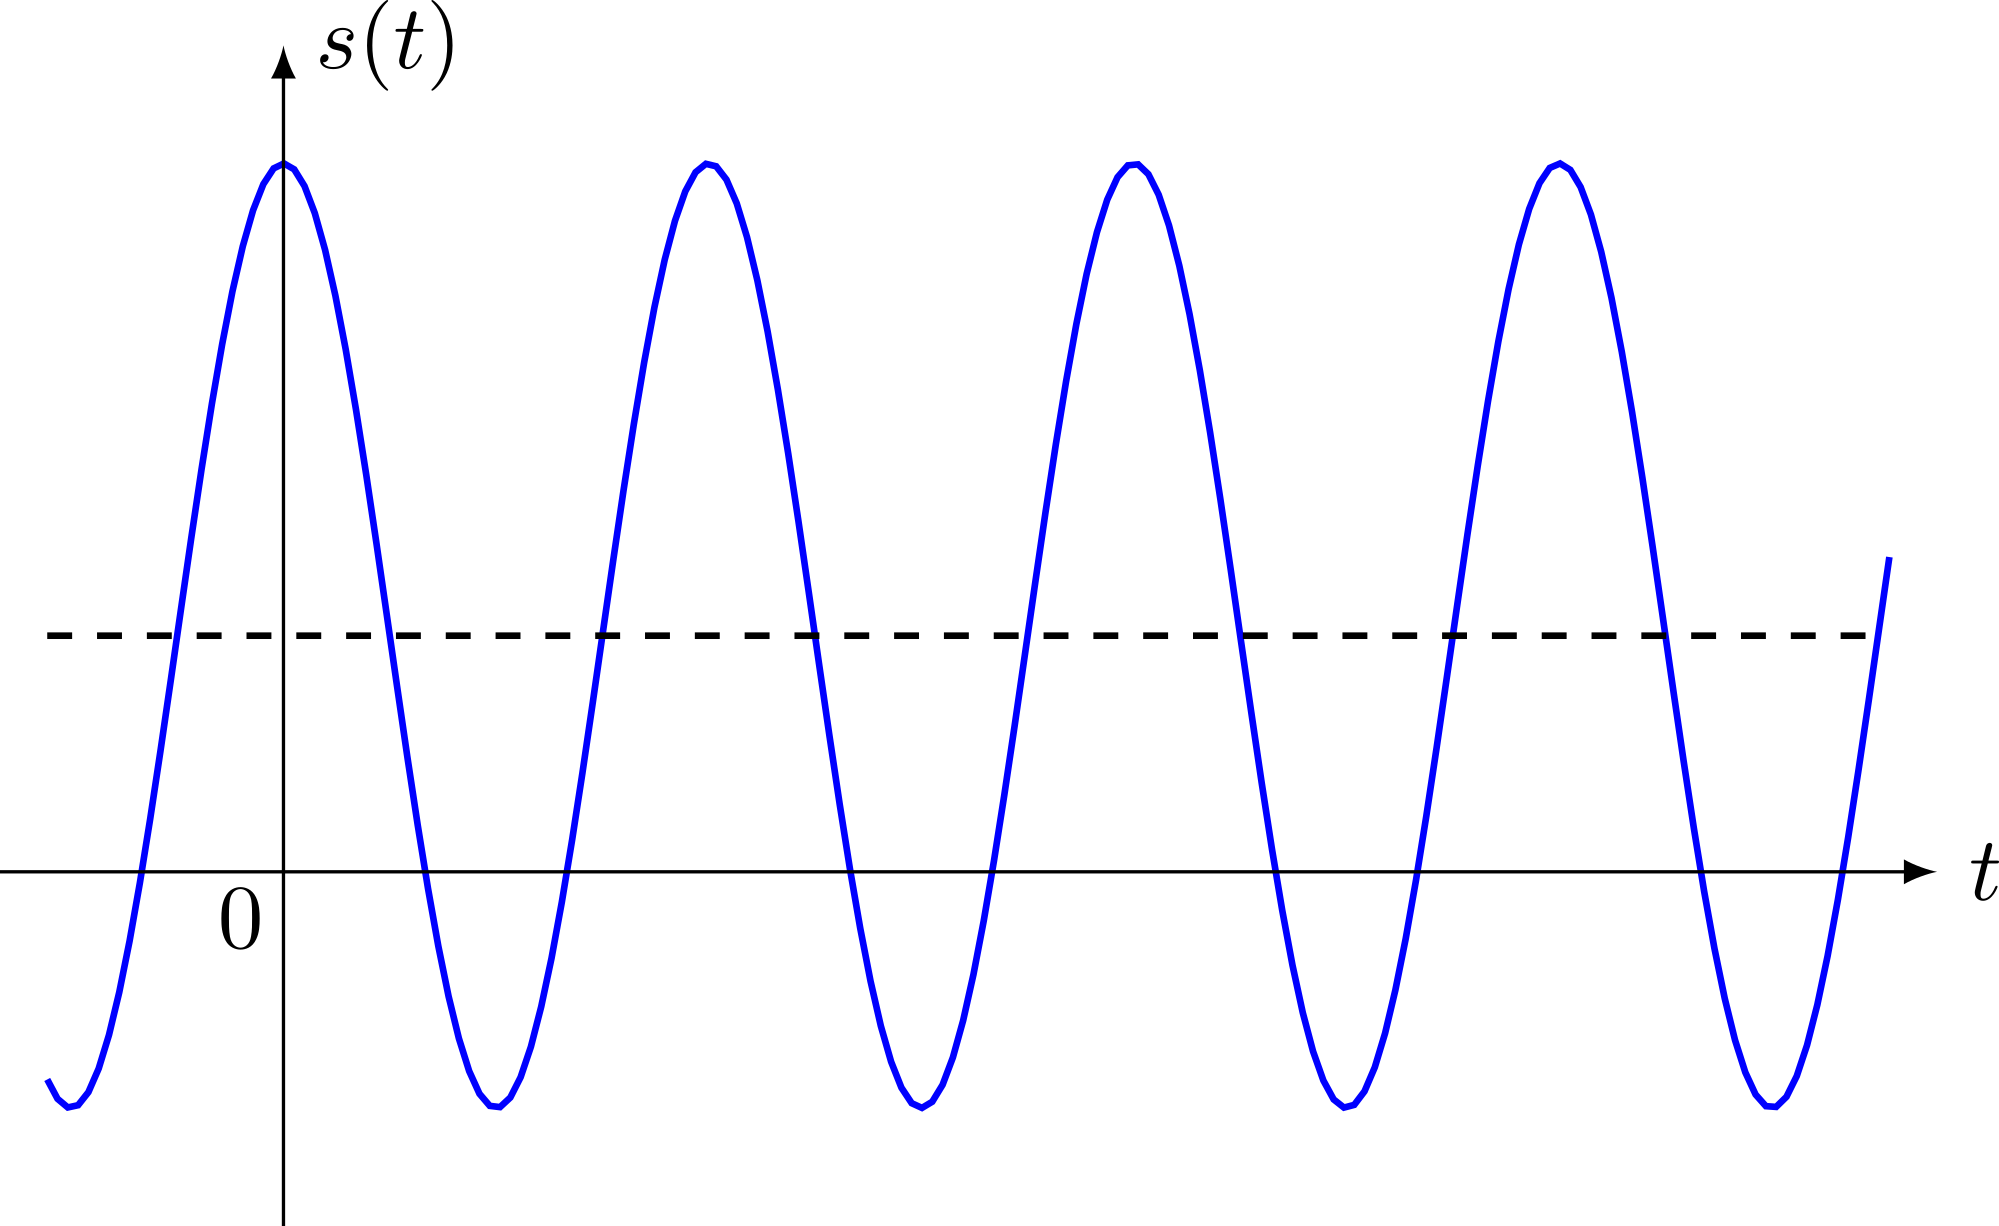
\includegraphics[width=\linewidth]{moy_cos-S0}
		\captionof{figure}{$s(t) = S_0 + A\cos(\wt)$}
	\end{center}
	\tcblower
	\psw{
		\begin{align*}
			\moy{s(t)}         & =
			\frac{1}{T} \int_{0}^{T} (S_0 + A\cos(\wt))\dd{t}
			\\&=
			\frac{1}{T} \left( \int_{0}^{T} S_0 \dd{t} +
			\int_{0}^{T} A \cos(\wt)\dd{t} \right)
			\\&=
			\frac{1}{T} \left( [S_0t]_0^{T} +
			\left[ \frac{A}{\w} \sin(\wt) \right]_0^{T} \right)
			\\&=
			\frac{1}{T} \left( S_0(T-0) +
			\underbracket[1pt]{\frac{A}{\w} \left( \sin(\w T) - \sin(\w \times 0) \right)}_{=0} \right)
			\\&=
			\frac{1}{T} S_0T
			\\\Lra
			\Aboxed{\moy{s(t)} & = S_0}
			\qed
		\end{align*}
	}
	\vspace{-15pt}
\end{tcb*}
\begin{tcb*}[cnt, bld](ror){Moyenne d'un signal sinusoïdal}
	Un signal purement sinusoïdal a une moyenne nulle.
\end{tcb*}

\subsection{Valeur efficace}
Ainsi, si on envoie une tension sinusoïdale dans un circuit et qu'on mesure la
moyenne de la tension reçue, on trouvera une tension nulle. Pourtant, l'énergie
transmise n'est pas nulle~! C'est parce que les électrons réagissent à la fois
aux tensions positives et négatives du signal, et ce pourquoi on obtient $\Ec_C
	= \frac{1}{2}Cu_C{}^{2}$~: l'\textbf{énergie est propotionnelle au carré des
	signaux}.
\begin{tcb*}(defi){Valeur efficace}
	On définit la valeur efficace d'un signal \textbf{périodique} par
	\psw{
		\[
			s \ind{eff} = \sqrt{\moy{s^{2}(t)}}
		\]
	}
	\vspace{-15pt}
\end{tcb*}
Ainsi, $s \ind{eff}^{2}$ représente l'énergie moyenne. Notamment, la valeur de
\SI{230}{V} pour la tension secteur est la valeur \textit{efficace}~: c'est une
tension sinusoïdale qui oscille entre des valeurs de $\SI{\pm 325}{V}$.

\begin{tcb*}[sidebyside, lefthand ratio=.4](appl){Calcul de valeur efficace}
	Calculer la valeur efficace du signal
	\[
		s(t) = A \cos(\wt)
	\]
	\begin{center}
		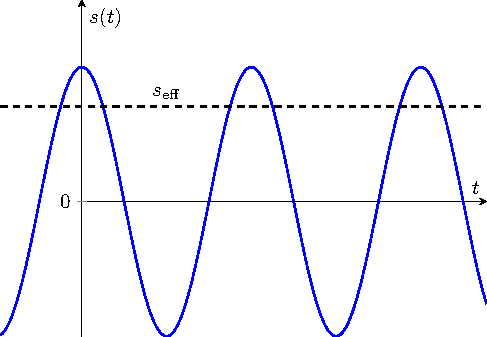
\includegraphics[width=\linewidth]{veff_cos}
		\captionof{figure}{$s \ind{eff}$ de $A\cos(\wt)$.}
	\end{center}
	\tcblower
	\psw{
		\begin{align*}
			\moy{s^{2}(t)}      & =
			\frac{1}{T} \int_{0}^{T} \left( A^{2}\cos^{2}(\wt) \right) \dd{t}
			\\ &=
			\frac{A^{2}}{T} \left( \int_{0}^{T} \frac{1}{2} \dd{t} +
			\int_{0}^{T} \frac{\cos(2\wt)}{2} \dd{t}\right)
			\\ &=
			\frac{A^{2}}{T}
			\Bigg(
			\underbracket[1pt]{\left[ \frac{1}{2}t \right]_0^{T}}_{=\frac{T}{2}} +
			\underbracket[1pt]{\left[ \frac{1}{2} \frac{A}{2\w} \sin(2\wt) \right]_0^{T}}_{=0}
			\Bigg)
			\\[-18pt] &=
			\frac{A^{2}}{2}
			\\\Lra
			\Aboxed{s \ind{eff} & = \frac{A}{\sqrt{2}}}
			\qed
		\end{align*}
	}
\end{tcb*}

\begin{tcb*}(impo)<lfnt>{Rapport $\sqrt{2}$}
	Il n'y a pas toujours de rapport $\sqrt{2}$ entre amplitude et valeur
	efficace~! Pour un signal triangle, la valeur efficace est $A/\sqrt{3}$, et
	pour un créneau pur sa valeur efficace est son amplitude $A$.
\end{tcb*}

\section{Décomposition en série de \textsc{Fourier}}
Le traitement de signal complexe a pu émerger grâce à un des théorèmes les plus
importants de la physique dans sa totalité, le théorème de \textsc{Fourier}.
Pour une introduction visuelle et des analyses de qualité, je vous recommande
les vidéos de \textsc{3Blue1Brown} portant sur le
sujet\footnote{%
	\href{https://www.youtube.com/watch?v=spUNpyF58BY}%
	{Mais qu'est-ce que la Transformée de Fourier~? Une introduction visuelle.}
}\footnote{%
	\href{https://www.youtube.com/watch?v=r6sGWTCMz2k}%
	{Mais qu'est-ce qu'une série de Fourier? Du transfert thermique à des
		dessins avec des cercles.}}. Pour
une approche un peu plus historique et concernant l'importance de l'algorithme
informatique basé sur ce théorème, je vous recommande la vidéo de
\textsc{Veritasium}\ftn{\href{https://www.youtube.com/watch?v=nmgFG7PUHfo}{The
		Remarkable Story Behind The Most Important Algorithm Of All Time}}.
\vspace{-15pt}
\subsection{Théorème de \textsc{Fourier}}
\begin{tcb*}[breakable](theo){\textsc{Fourier}}
	Tout signal périodique se décompose comme une somme, éventuellement infinie,
	de fonctions sinusoïdales. Ainsi, un signal périodique complexe $s(t)$ de
	pulsation $\w$ s'écrit
	\psw{
		\[
			s(t) = S_0 + \sum_{n=1}^{+\infty} S_n \cos(n\w t + \f_n)
			\Lra
			s(t) = S_0 + \sum_{n=1}^{+\infty} S_n \cos(2\pi nf t + \f_n)
		\]
	}%
	Avec $S_0$ la valeur moyenne (composante continue), et les $S_n$ et $\f_n$ des
	caractéristiques du signal. Les amplitudes $S_n$ constituent le
	\textbf{spectre} du signal.
\end{tcb*}
% \tikz[remember picture, overlay]
% \draw[-stealth, transform canvas={xshift=-6pt, yshift=-6pt}]
% (pic cs:so) --++ (-10pt,-10pt)
% node[anchor=north] {moyenne}
%~;
% \tikz[remember picture, overlay]
% \draw[-stealth, transform canvas={xshift=-3pt, yshift=-6pt}]
% (pic cs:sk) --++(0pt,-10pt)
% node[anchor=north] {composantes}
%~;
% \tikz[remember picture, overlay]
% \draw[-stealth, transform canvas={xshift=0pt, yshift=-6pt}]
% (pic cs:fk) --++(5pt,-10pt)
% node[anchor=north] {phases}
%~;

\subsection{Analyse spectrale}
% Olivier

\noindent
\begin{minipage}[t]{.48\linewidth}
	Le \textbf{spectre} d'un signal représente l'amplitude des différentes
	composantes sinusoïdales le constituant en fonction de leurs
	\textbf{fréquences}. Il donne les fréquences et les importances relatives des
	sinus.
	\begin{tcb}(nota){Fondamental et harmoniques}
		\begin{itemize}
			\item La première composante sinusoïdale, $S_1 \cos(\wt + \f_1)$,
			      s'appelle le \textbf{fondamental}. Il \textbf{donne sa fréquence au
				      signal entier}.
			\item Le signal $S_n \cos(n\wt + \f_n)$ est appellé
			      \textbf{harmonique de rang $\mathbf{n}$}. Sa pulsation est un
			      \textbf{multiple} du fondamental.
		\end{itemize}
	\end{tcb}
\end{minipage}
\hfill
\begin{minipage}[t]{.48\linewidth}
	\vspace{-10pt}
	\begin{center}
		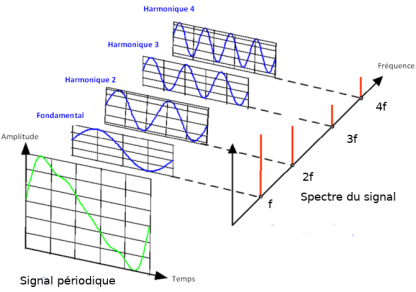
\includegraphics[width=\linewidth]{decompo_fourier}
		\captionof{figure}{Décomposition de \textsc{Fourier} d'un signal complexe
			\protect\ftn{Pour un approche ludique, essayer ce site~:
				\href{https://phet.colorado.edu/sims/html/fourier-making-waves/latest/fourier-making-waveS_en.html}
				{Composeur de séries de \textsc{Fourier}}}.}
		\label{fig:fourier}
	\end{center}
\end{minipage}

% \begin{figure}[htbp!]
% 	\centering
% 	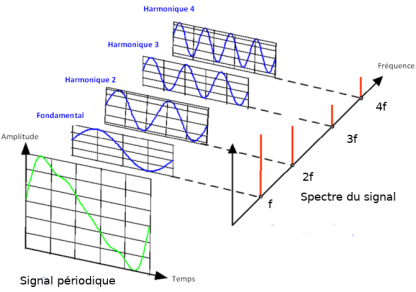
\includegraphics[scale=1]{decompo_fourier.png}
% 	\caption{Décomposition de \textsc{Fourier} d'un signal complexe.}
% 	\label{fig:fourier}
% \end{figure}

\begin{tcb*}[breakable](exem){Décompositions en séries de \textsc{Fourier}}
	\begin{minipage}{\linewidth}
		\centering
		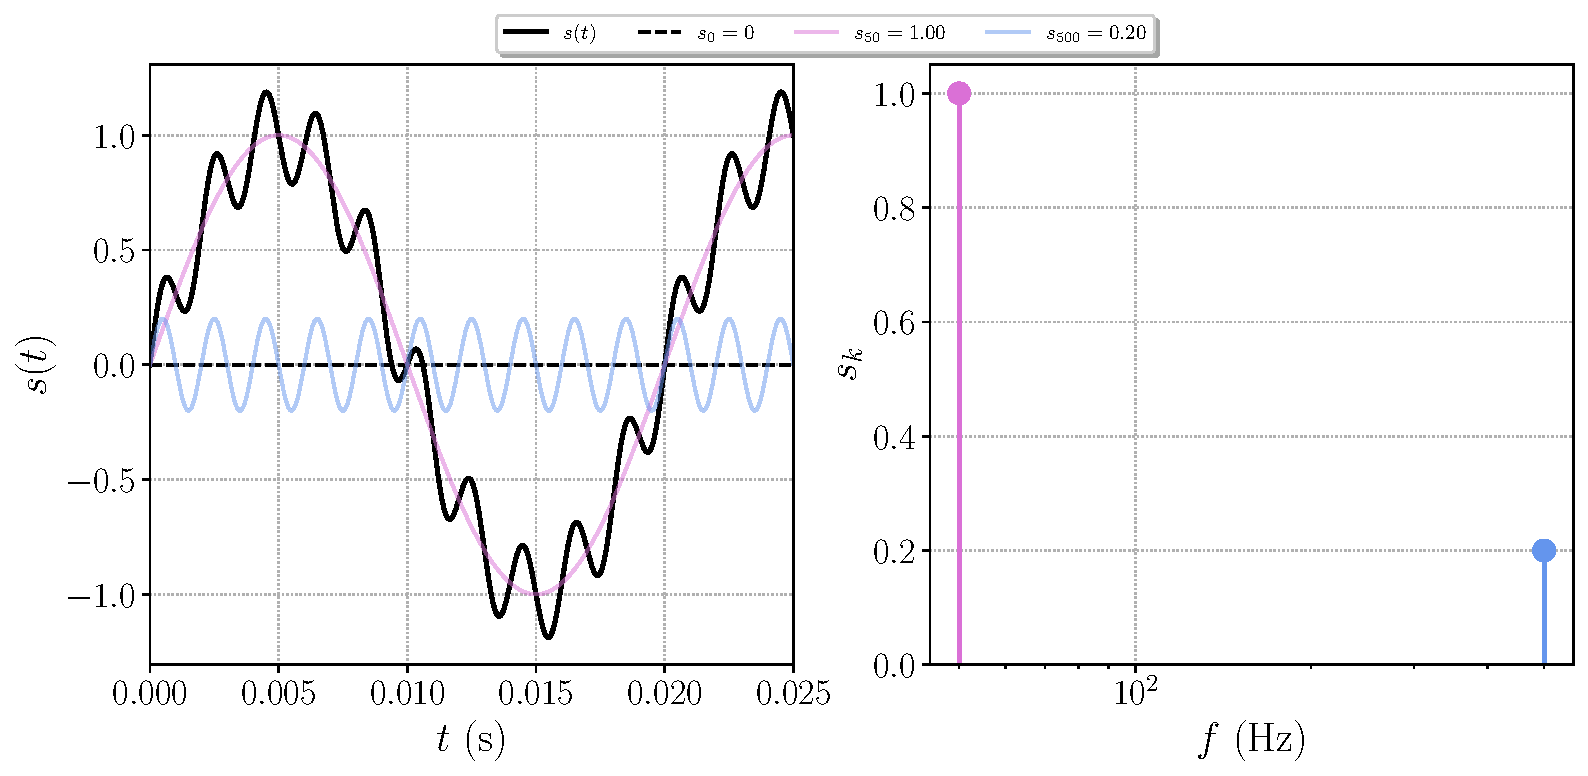
\includegraphics[width=.85\linewidth]{fft_50_[1,10]_[1,0.2]}
		\captionof{figure}{Signal somme de 50 et \SI{500}{Hz}}
	\end{minipage}

	\begin{minipage}{\linewidth}
		\centering
		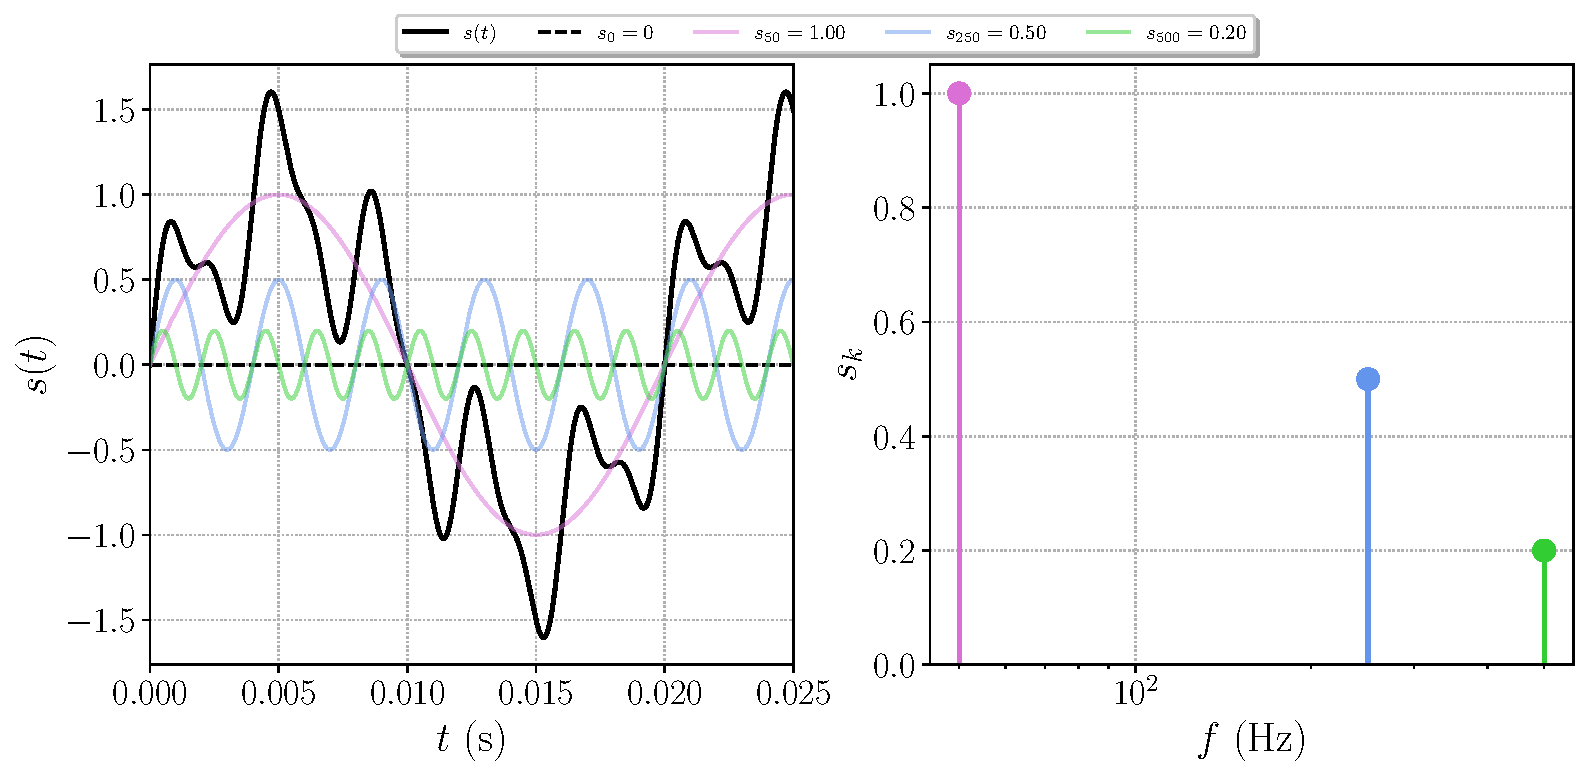
\includegraphics[width=.85\linewidth]{fft_50_[1,5,10]_[1,0.5,0.2]}
		\captionof{figure}{Signal somme de 50, 250 et \SI{500}{Hz}}
		\label{fig:3some}
	\end{minipage}

	\begin{minipage}{\linewidth}
		\centering
		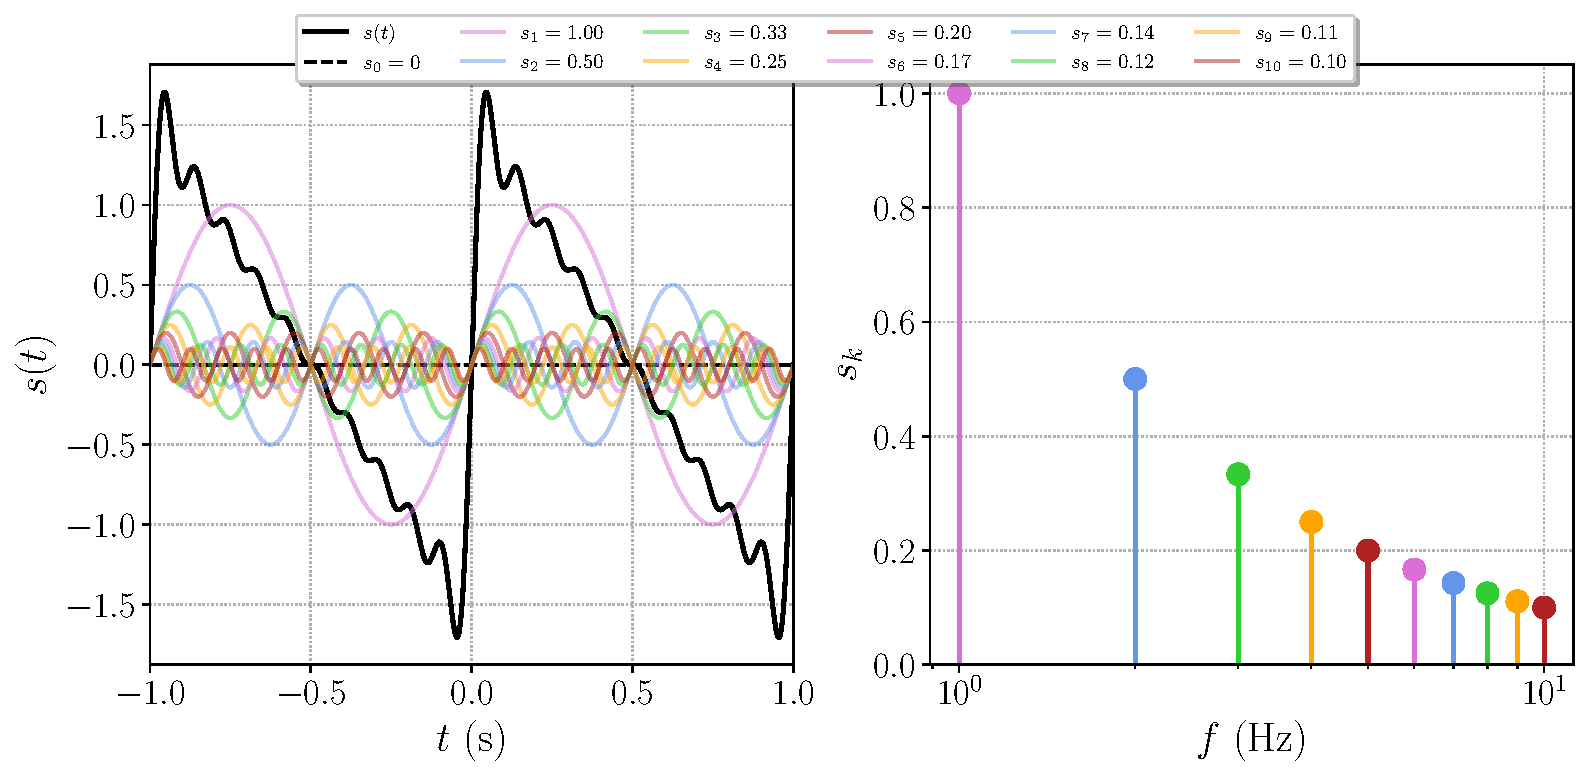
\includegraphics[width=.85\linewidth]{fft_add}
		\captionof{figure}{Signal rampe~: $S_k = 1/k$}
	\end{minipage}

	\begin{minipage}{\linewidth}
		\centering
		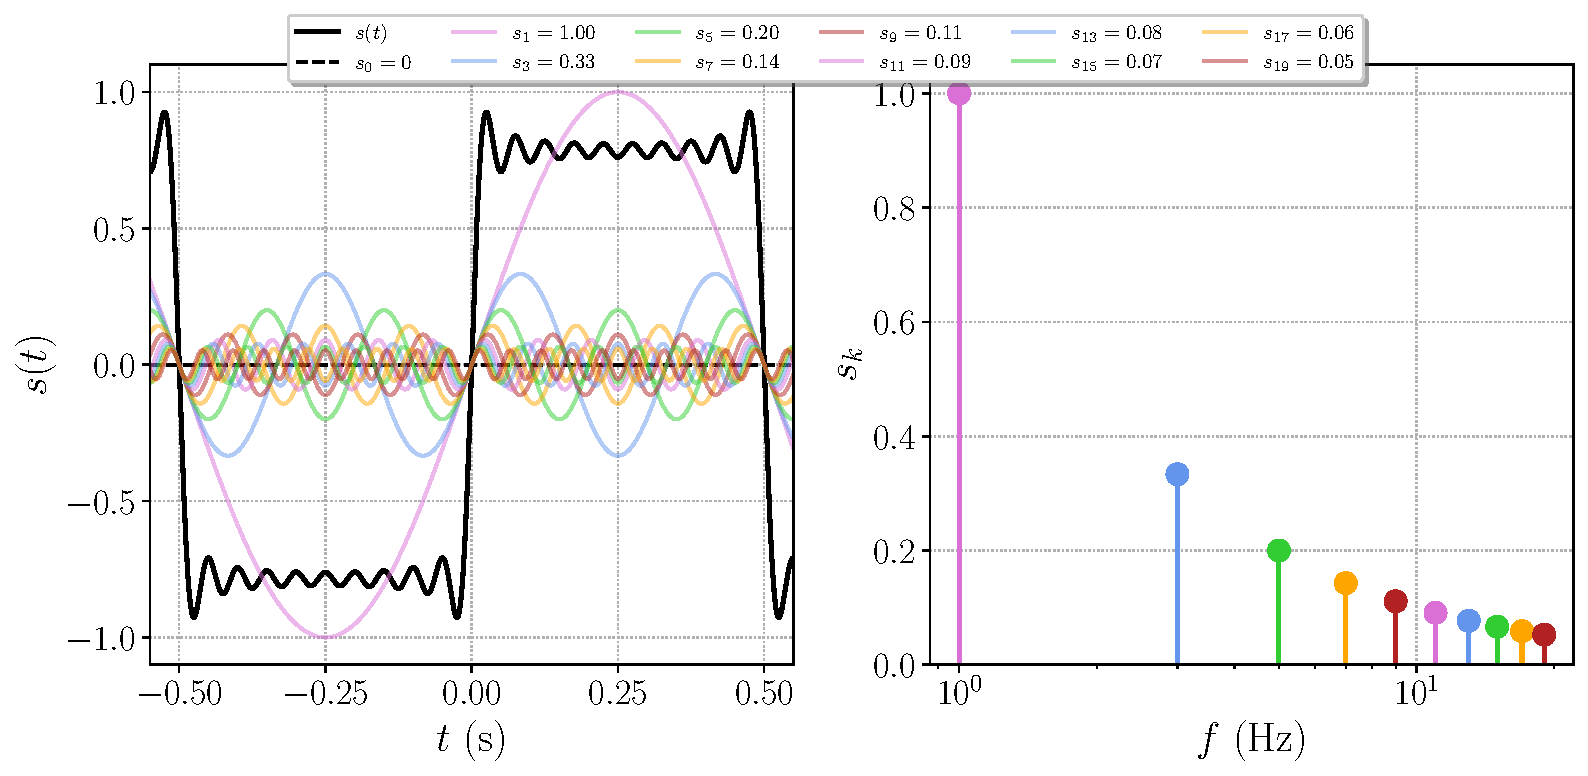
\includegraphics[width=.85\linewidth]{fft_creneau}
		\captionof{figure}{Signal créneau~: $S_{2k+1} = 1/(2k+1)$}
	\end{minipage}
\end{tcb*}

\begin{tcb*}(rema){Hautes et basses fréquences}
	\begin{itemize}
		\item Les \textbf{basses fréquences} «~codent~» les \textbf{variations
			      lentes} d'un signal~;
		\item les \textbf{hautes fréquences} «~codent~» les \textbf{variations
			      brusques} d'un signal.
	\end{itemize}
\end{tcb*}

\subsection{Relation de \textsc{Parseval}}
Si l'on peut décomposer tout signal en somme de sinus, et que l'énergie moyenne
d'une fonction sinusoïdale est $\moy{s^{2}(t)}$, alors on peut espérer que
l'énergie de tout le signal est la somme des fréquences individuelles  le
composant. C'est en effet le cas~:
\begin{tcb*}(prop){Relation de \textsc{Parseval}}
	\psw{
	\[
		\moy{s^{2}(t)} = s^{2}\ind{eff} =
		S_0{}^{2} + \frac{1}{2} \sum_{n=1}^{+\infty} S_n{}^{2}
	\]
	}
	Ainsi, l'énergie portée par un signal se répartit dans ses harmoniques, et ce
	de façon indépendante.
\end{tcb*}

\section{Filtrage}
\subsection{Traitement du signal et filtre}
Le but du \textbf{traitement du signal} est d'\textbf{extraire l'information
	utile} d'un signal issu d'un capteur où de multiples signaux se superposent au
signal utile~: bruits électromagnétiques, autres informations, etc.
\begin{itemize}
	\item Pour recevoir la radio, on doit sélectionner le signal autour d'une
	      bande de fréquence précise et éliminer le reste~;
	\item Pour isoler une voix dans un morceau de musique, c'est le même principe.
\end{itemize}

\begin{tcb*}[sidebyside, righthand ratio=.3](defi){Filtre}
	Système qui \textbf{traite un signal} sur un \textbf{critère fréquentiel}. On
	le représente par un \textbf{quadripôle} dans les schémas électrique, avec
	$e(t)$ l'entrée et $s(t)$ la sortie. On en distingue 3 types principaux~:
	\begin{itemize}
		\bitem{Passe-bas}~: ne laisse passer que les basses fréquences~;
		\bitem{Passe-haut}~: ne laisse passer que les hautes fréquences~;
		\bitem{Passe-bande}~: ne laisse passer qu'une bande de fréquences.
	\end{itemize}
	Il est dit \textbf{linéaire} si la sortie est de même(s) fréquence(s) que
	l'entrée (i.e., l'équation différentielle derrière son action est une EDL).
	\tcblower
	\begin{center}
		\sswitch{
			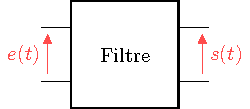
\includegraphics[width=\linewidth, draft=true]{filtre_plain}
		}{
			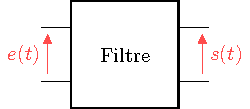
\includegraphics[width=\linewidth]{filtre_plain}
		}
		\captionof{figure}{Filtre.}
	\end{center}
\end{tcb*}

\subsection{Fonction de transfert d'un filtre}

La grandeur caractérisant l'action d'un filtre est sa \textbf{fonction de
	transfert}~:
\begin{tcb*}(defi){Fonction de transfert}
	C'est la grandeur complexe
	\psw{
		\[
			\Hu = \frac{\Su}{\Eu}
			\Lra
			\Su = \Hu\Eu
		\]
	}
	avec $\Su$ l'amplitude complexe du signal de sortie, et $\Eu$ celle du signal
	d'entrée.
\end{tcb*}
Pour un filtre linéaire, la fonction de transfert s'applique à chaque sinusoïde
du signal d'entrée pour donner une sinusoïde de sortie~:
\psw{
	\[
		e_n(t) = E_n \sin(n\w_e t + \f_n)
		\Ra
		s_n(t) = S_n \sin(n\w_e t + \psi_n)
	\]
}
et on trouve l'amplitude réelle et la phase réelle de sortie en prenant le
module et l'argument de $\Su$, soit
\psw{
	\[
		S_n = \abs{\xul{S_n}} = \abs{\xul{H}\xul{E_n}}
		\qet
		\psi_n = \arg*{{\xul{S_n}}} = \arg*{{\xul{H}\xul{E_n}}}
	\]
}

Nous avons, sans le mentionné, déjà rencontré et manipulé des filtres. Le premier
exemple est celui du filtre RC~:
\begin{tcbraster}[raster columns=2, raster equal height=rows]
	\begin{tcb}(exem)<lfnt>'l'{Exemple}
		\begin{minipage}{\linewidth}
			\sswitch{
				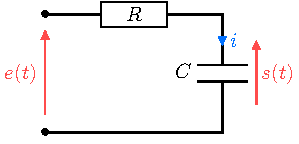
\includegraphics[width=\linewidth, draft=true]{filtre_rc}
			}{
				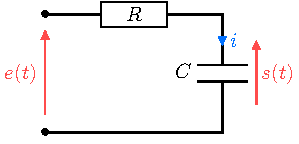
\includegraphics[width=\linewidth]{filtre_rc}
			}
			\vspace{-15pt}
			\captionof{figure}{Filtre RC.}
		\end{minipage}
	\end{tcb}
	\begin{tcb}(impo)<rgnt>'r'{Attention}
		On n'indique pas le reste du circuit, mais \textbf{un filtre s'insère
			dans un circuit}~:
		\begin{itemize}
			\item $e(t)$ peut venir d'un générateur, d'un amplificateur, etc.
			\item $s(t)$ peut aller vers un appareil de mesure, un haut-parleur,
			      etc.
		\end{itemize}
	\end{tcb}
\end{tcbraster}

Pour trouver la fonction de transfert, on transforme le circuit en complexes et
on applique un pont diviseur de tension~:
\smallbreak
\noindent
\begin{minipage}[c]{.45\linewidth}
	\begin{center}
		\sswitch{
			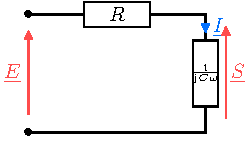
\includegraphics[width=\linewidth, draft=true]{filtre_rc-cplx}
		}{
			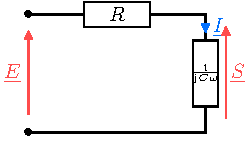
\includegraphics[width=\linewidth]{filtre_rc-cplx}
		}
		\vspace{-15pt}
		\captionof{figure}{RC en complexes.}
	\end{center}
\end{minipage}
\hfill
\begin{minipage}[c]{.5\linewidth}
	Pont diviseur~:
	\psw{
		\begin{DispWithArrows*}[fleqn, mathindent=-5pt]
			\Su &= \frac{1/\jcw}{R + 1/\jcw}\Eu
			\CArrow{$\times \frac{\jcw}{\jcw}$}
			\\\Lra
			\Su &= \frac{1}{1+\jrcw}\Eu
			\Arrow{$\Hu = \Su/\Eu$}
			\\\Lra
			\Aboxed{\Hu &= \frac{1}{1+\jrcw} = \frac{1}{1+\jj \frac{\w}{\w_c}}}
		\end{DispWithArrows*}
		avec $\w_c = \frac{1}{RC}$ la pulsation de coupure
	}
\end{minipage}

\begin{tcb*}(nota){Pulsation réduite}
	Pour alléger les notations, et se ramener à des grandeurs centrées autour de
	l'unité, il est commode d'introduire la \textbf{pulsation réduite}~:
	\psw{
		\[
			x = \frac{\w}{\w_c}
		\]
	}
	Ainsi, pour le RC, on obtient pour $\Hu$~:
	\psw{
		\[
			\Hu(x) = \frac{1}{1+\jx}
		\]
	}
	\vspace{-15pt}
\end{tcb*}

\subsection{Effet d'un filtre sur un signal périodique}

L'objectif de ce chapitre est de comprendre comment un filtre impacte un signal
périodique quelconque, décomposable en signaux sinusoïdaux. L'idée est semblable
à ce qu'on a fait au chapitre précédent~; en effet, grâce à la linéarité du
filtre, on procède par superposition~:
\begin{enumerate}
	\item On décompose le signal d'entrée en sinusoïdes, avec $\w_e$ la pulsation
	      d'entrée du fondamental et $\w_n = n\w_e$ les pulsations des harmoniques~:
	      \psw{
		      \[
			      e(t) = E_0 + \sum_{n=1}^{+\infty} E_n \sin(\w_n t + \f_n)
		      \]
	      }
	      \vspace{-15pt}
	\item On applique la fonction de transfert à chaque entrée sinusoïdale pour
	      obtenir les sorties correspondantes~:
	      \psw{
		      \[
			      s_n(t) = S_n \sin(\w_n t + \psi_n)
			      \qav
			      S_n = E_n \times \abs{\Hu(\jw_n)}
			      \qet
			      \psi_n = \f_n + \arg*{\Hu(\jw_n})
		      \]
	      }
	      \vspace{-15pt}
	\item On recompose le signal de sortie en sommant les sorties obtenues~:
	      \psw{
		      \[
			      s(t) = \sum_{n=0}^{+\infty}s_n(t)
		      \]
	      }
	      \vspace{-15pt}
\end{enumerate}

\[
	e(t) =
	\left\{
	\begin{array}{ccccc}
		E_0                     & \ra & \fbox{$\Hu(0\jw_e)$} & \ra & S_0
		\\
		+                       &     &                      &     & +
		\\
		E_1\sin(\w_e t + \f_1)  & \ra & \fbox{$\Hu(1\jw_e)$} & \ra & S_1\sin(\w_e t + \psi_1)
		\\
		+                       &     &                      &     & +
		\\
		E_2\sin(2\w_e t + \f_2) & \ra & \fbox{$\Hu(2\jw_e)$} & \ra & S_2\sin(2\w_e t + \psi_2)
		\\
		\vdots                  &     &                      &     & \vdots
		\\
		E_n\sin(n\w_e t + \f_n) & \ra & \fbox{$\Hu(n\jw_e)$} & \ra & S_n\sin(n\w_e t + \psi_n)
	\end{array}
	\right\} = s(t)
\]

% Olivier + Corot p.19

\section{Description d'un filtre}
Pour représenter ces actions, outre la forme analytique d'un filtre, on définit
des grandeurs utiles et on met en place des représentations pertinentes.

\subsection{Gain et gain en décibels}
\begin{tcb*}(defi){Gains}
	\begin{enumerate}
		\item Le \textbf{gain} traduit l'effet du filtre sur l'amplitude d'un
		      signal, et on a
		      \psw{
			      \[
				      \boxed{G(x) = \abs{\Hu(x)} = \frac{S_n(x)}{E_n}}
			      \]
		      }
		      Le gain est sans unité, sans dimension.
		      \begin{itemize}
			      \item $G(x) = 1 \Ra S_n(x) = E_n$~: signal d'entrée conservé à cette
			            fréquence.
			      \item $G(x) > 1 \Ra S_n(x) > E_n$~: signal d'entrée amplifié à cette
			            fréquence.
			      \item $G(x) < 1 \Ra S_n(x) < E_n$~: signal d'entrée atténué à cette
			            fréquence.
		      \end{itemize}
		\item Le \textbf{gain en décibel} (\si{dB}) traduit le même effet, mais en
		      échelle logarithmique~:
		      \psw{
			      \[
				      \boxed{G\ind{dB}(x) = 20 \log \abs{\Hu(x)}}
			      \]
		      }
		      Le gain en décibels a pour unité le \si{dB}.
		      \begin{itemize}
			      \item $G\ind{dB}(x) = \SI{0}{dB} \Lra \abs{\Hu(x)} = 1$~: signal
			            d'entrée conservé à cette fréquence.
			      \item $G\ind{dB}(x) > \SI{0}{dB} \Lra \abs{\Hu(x)} > 1$~: signal
			            d'entrée amplifié à cette fréquence.
			      \item $G\ind{dB}(x) < \SI{0}{dB} \Lra \abs{\Hu(x)} < 1$~: signal
			            d'entrée atténué à cette fréquence.
		      \end{itemize}
	\end{enumerate}
\end{tcb*}
En effet, les échelles logarithmiques sont utiles pour visualiser des données
sur de grands intervalles.
\smallbreak
\noindent
\begin{minipage}{\linewidth}
	\centering
	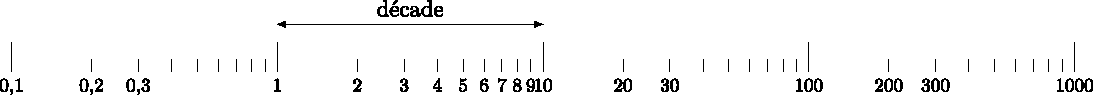
\includegraphics[width=\linewidth]{logscale}
	\captionof{figure}{Exemple d'échelle logarithmique}
	\label{fig:logscale}
\end{minipage}

À l'inverse d'une échelle linéaire, ici les incréments sont des
\textbf{puissances de 10}. Le passage d'une puissance de 10 à la suivante
s'appelle une \textbf{décade}.

\begin{tcb*}(rapp)<lfnt>{Logarithme décimal}
	Le logarithme décimal est la fonction inverse de la fonction $f:x\mapsto
		10^{x}$. Ainsi,
	\[
		\log(10^{1}) = 1
		\quad~; \quad
		\log (10^{2}) = 2
		\quad~; \quad
		\log (10^{3}) = 3
	\]
\end{tcb*}

\begin{tcb*}(prop){Amplitude vs.\ gain}
	\begin{enumerate}
		\item Lorsque l'\textbf{amplitude est divisée par 10}, le \textbf{gain en
			      décibels diminue de \SI{20}{dB}}~;
		\item La bande passante est l'ensemble des pulsations telles que
		      $G\ind{dB}(\w) \geq G\ind{dB,max} - \SI{3}{dB}$~:
		      \[
			      \text{bande passante}
			      \quad \triangleq \quad
			      \{\w ~|~ G\ind{dB}(\w) \geq G\ind{dB, max}-\SI{3}{dB}\}
		      \]
	\end{enumerate}
\end{tcb*}
\begin{tcb*}[sidebyside](demo){Amplitude vs.\ gain}
	\begin{enumerate}
		\mitem
		\psw{
			\small
			\begin{align*}
				\abs{\Hu(\w_2)}                        & = \frac{\abs{\Hu(\w_1)}}{10}
				\\\Lra
				20 \log \left( \abs{\Hu(\w_2)} \right) & =
				20 \log (\frac{\abs{\Hu(\w_1)}}{10})
				\\\Lra
				20 \log \left( \abs{\Hu(\w_2)} \right) & =
				20 \log (\abs{\Hu(\w_1)}) - 20 \log (10)
				\\\Lra
				G\ind{dB}(\w_2)                        & = G\ind{dB}(\w_1) - \SI{20}{dB}
				\qed
			\end{align*}
		}
		\vspace{-15pt}
	\end{enumerate}
	\tcblower
	\begin{enumerate}[start=2]
		\mitem
		\psw{
			\small
			\begin{align*}
				\abs{\Hu(\w)}           & \geq \frac{\abs{\Hu}_{\max}}{\sqrt{2}}
				\\\Lra
				20 \log (\abs{\Hu(\w)}) & \geq 20 \log (\frac{\abs{\Hu}_{\max}}{\sqrt{2}})
				\\\Lra
				G\ind{dB}(\w)           & \geq
				\underbracket[1pt]{20 \log (\abs{\Hu}_{\max})}_{= G\ind{dB, max}} -
				\underbracket[1pt]{20 \log (\sqrt{2})}_{= \SI{3}{dB}}
				\qed
			\end{align*}
			\vspace{-15pt}
		}
	\end{enumerate}
\end{tcb*}

\begin{tcb*}[breakable](appl){Gain du filtre RC sur C}
	On rappelle la fonction de transfert du filtre RC sur C~: $\Hu(x) =
		\frac{1}{1+\jx}$.
	\begin{enumerate}
		\item Déterminer son gain. Quel est son maximum~?
		\item En déduire son gain en décibels. Quel est son maximum~?
		\item Déterminer sa bande passante \textit{à l'aide du gain}.
		\item Déterminer sa phase. Donner ses limites pour $x\to 0$ et $x\to\infty$.
	\end{enumerate}
	\tcblower
	\vspace{12pt}
	\begin{enumerate}
		\mitem
		\psw{
		\[
			\boxed{G(x) = \abs{\Hu} = \frac{1}{\sqrt{1+x^{2}}}}
			\qet
			\xul{G_{\max} = G(0) = 1}
		\]
		}
		\mitem
		\psw{
			\begin{gather*}
				G\ind{dB}(x) = 20 \log (\sqrt{1+x^{2}}^{-1}) = \frac{20}{-2} \log
				(1+x^{2})
				\\\Lra
				\boxed{G\ind{dB}(x) = -10 \log (1+x^{2})}
				\Ra
				\xul{G\ind{dB, max} = 0}
			\end{gather*}
		}
		\mitem
		\psw{
			\begin{gather*}
				G(x) \geq \frac{G\ind{max}}{\sqrt{2}}
				\Lra
				\frac{1}{\sqrt{1+x^{2}}} \geq \frac{1}{\sqrt{2}}
				\\\Lra
				\boxed{x \leq 1 \Lra \w \leq \w_c}
			\end{gather*}
		}
		\vspace*{-15pt}
		\item
		      \psw{
			      \begin{gather*}
				      \f(x) = \arg*{\Hu(x}) = -\arg*{ 1+\jx }
				      \Lra
				      \boxed{\f(x) = -\arctan(x)}
				      \\\Ra
				      \f(x) \opto{}{x\to 0} 0
				      \qet
				      \f(x) \opto{}{x\to\infty} -\frac{\pi}{2}
			      \end{gather*}
		      }
	\end{enumerate}
\end{tcb*}

\subsection{Diagramme de \textsc{Bode}}

\subsubsection{Définition}
\begin{tcb*}(defi){Diagramme de \textsc{Bode}}
	Le(s) diagramme(s) de \textsc{Bode} est un outil permettant de visualiser
	\textit{et quantifier} l'effet d'un filtre sur une fréquence d'entrée. On
	représente pour cela~:
	\begin{itemize}
		\item \textbf{gain en décibels} $G\ind{dB}(x) = 20 \log \abs{\Hu(x)}$~;
		\item et sa \textbf{phase} $\f(x) = \arg*{{\Hu(x}})$.
	\end{itemize}
	\smallbreak
	On les trace en fonction de la pulsation (réduite ou non) ou de la fréquence,
	et \textbf{en échelle logarithmique}.
\end{tcb*}
Par exemple, pour le RC sur C~:
\begin{figure}[htbp!]
	\centering
	\subcaptionbox{Gain}[.48\linewidth]
	{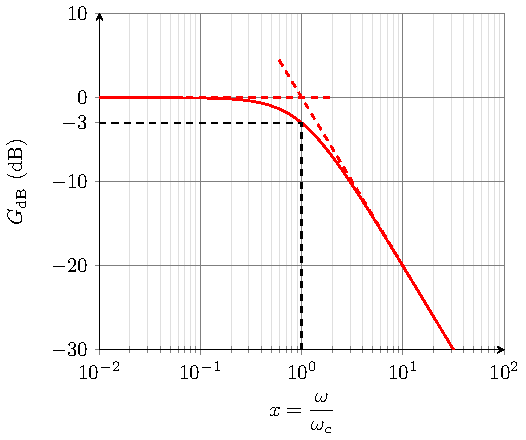
\includegraphics[width=\linewidth]{RCC_bode-gain}}
	\subcaptionbox{Phase}[.48\linewidth]
	{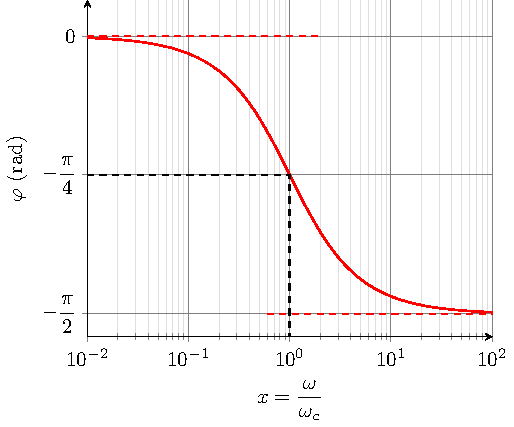
\includegraphics[width=\linewidth]{RCC_bode-phase}}
	\caption{Diagramme de \textsc{Bode} du filtre RC sur C.}
	\label{fig:rccbode_first}
\end{figure}
C'est donc un \textbf{passe-bas}~!
% \begin{center}
% 	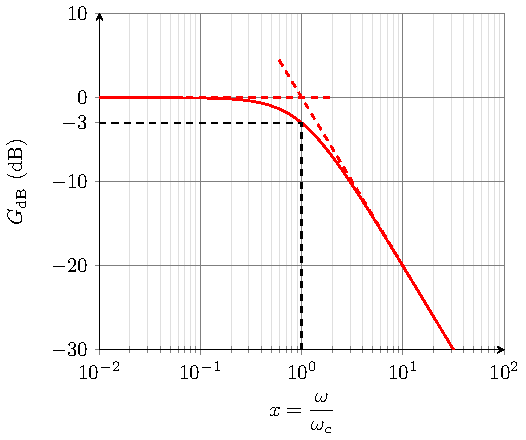
\includegraphics[width=0.48\linewidth]{RCC_bode-gain}
% 	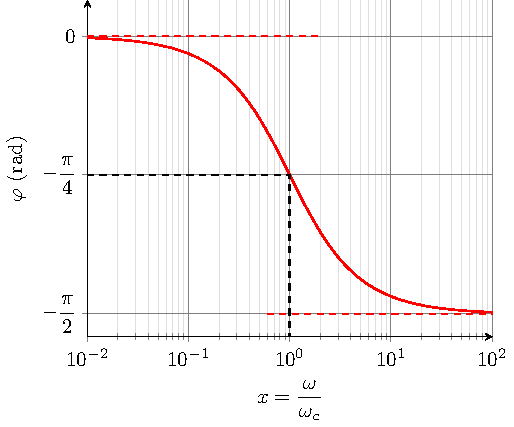
\includegraphics[width=0.48\linewidth]{RCC_bode-phase}
% \end{center}

\subsubsection{Asymptotes}
\begin{tcb*}(defi){Diagramme asymptotique}
	Le diagramme de Bode asymptotique d'un filtre correspond au diagramme de Bode
	où seules les droites asymptotes affines sont tracées.
\end{tcb*}
\begin{tcb*}(tool){Obtention des asymptotes}
	Pour trouver les asymptotes~:
	\begin{enumerate}
		\item On simplifie $\Hu(x)$ pour $x\to 0$ et $x\to \infty$, en ne gardant
		      \textbf{que le terme prépondérant} au numérateur et au dénominateur~;
		\item On calcule $G\ind{dB}$ et $\f$ avec ces limites asymptotiques~;
		\item On trace les droites obtenues en les faisant se rejoindre.
	\end{enumerate}
\end{tcb*}
\begin{tcb*}(appl){Diagramme asymptotique RC sur C}
	Déterminer les droites asymptotes du diagramme de Bode de RC sur C. Vérifier
	la cohérence avec les asymptotique de la Figure~\ref{fig:rccbode_first}.
	\tcblower
	\vspace{12pt}
	\begin{enumerate}
		\mitem
		\psw{
			\[
				\boxed{
					\Hu(x) \opto{}{x\to 0} \frac{1}{1 + 0} = 1
					\qet
					\Hu(x) \opto{}{x\to \infty} \frac{1}{\jx}
				}
			\]
		}
		\vspace{-15pt}
		\item
		      \begin{itemize}
			      \item Pour le gain~:
			            \psw{
				            \[
					            G\ind{dB}(x) \opto{}{x\to 0} 20 \log (1) = 0
					            \qet
					            G\ind{dB}(x) \opto{}{x\to\infty} 20 \log \abs{\frac{1}{\jx}} = -20 \log
					            x
				            \]
			            }%
			            Ainsi, à hautes fréquences, \textbf{le gain diminue de
				            \SI{20}{dB} par décade}~: si $\w$ est multiplié par 10, le
			            gain en décibel baisse de \SI{20}{dB} (i.e.\ l'amplitude est
			            divisée par 10).
			      \item Pour la phase~:
			            \psw{
				            \[
					            \f(x) \opto{}{x\to 0} \arg*{1} = 0
					            \qet
					            \f(x) \opto{}{x\to \infty} \arg*{\frac{1}{\jx}} = -\frac{\pi}{2}
				            \]
			            }
			            \vspace{-15pt}
		      \end{itemize}
	\end{enumerate}
\end{tcb*}

% Corot p.7

\subsubsection{Lecture}
Pour lire le signal de sortie d'un filtre, il suffit de repérer le \textbf{gain}
et la \textbf{phase} de la fonction de transfert \textbf{pour chaque fréquence}
de la décomposition. Si $e(t) = E \cos(\wt)$, la sortie sera
\psw{
	\[
		s(t) = \abs{\Hu(\w)} \times E \cos(\wt + \f(\w))
	\]
}
On trouve le déphasage par lecture directe, et on trouve le gain à partir du
gain en décibel en inversant la formule~:
\psw{
	\[
		G\ind{dB}(\w) = 20 \log \abs{\Hu(\w)}
		\Lra
		\abs{\Hu(\w)} = 10^{G\ind{dB}(\w)/20}
	\]
}
\vspace{-15pt}
\begin{tcb*}(exem){Filtrage par RC sur C}
	En reprenant la Figure~\ref{fig:3some}, on ajoute le filtre RC en passe-bas.
	Pour garder les basses fréquences, on choisit une fréquence de coupure $f_c$ à
	\SI{10}{Hz}. Avec $R = \SI{1000}{\ohm}$ cela impose $C = \SI{1.6e-5}{F}$
	($\w_c = \frac{1}{RC}$). On obtient la figure suivante~:
	\smallbreak
	\noindent
	\begin{minipage}{\linewidth}
		\centering
		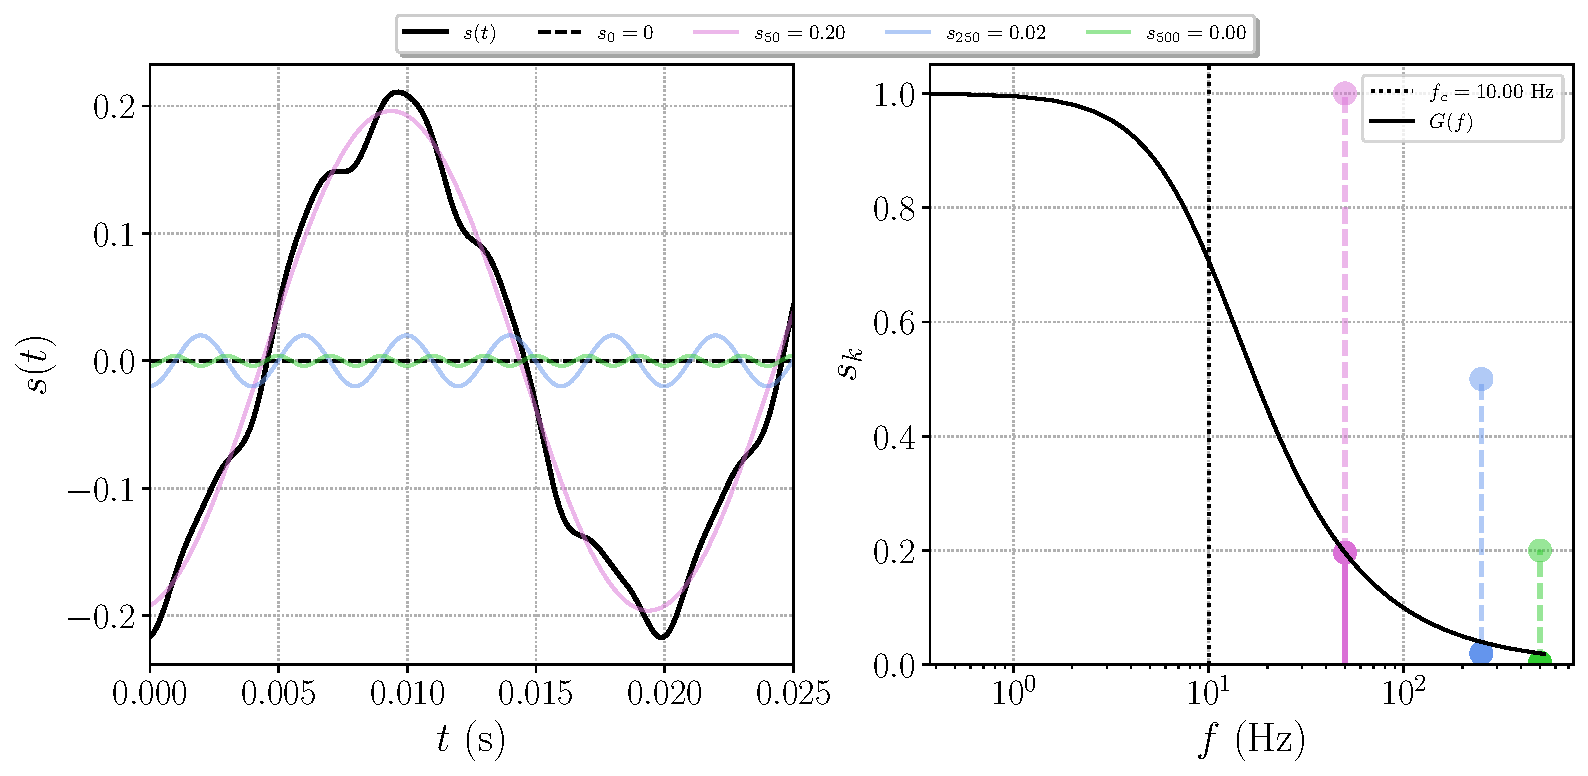
\includegraphics[width=.90\linewidth]{fft_50_[1,5,10]_[1,0.5,0.2]_fc=10}
		\captionof{figure}{Signal somme de 50, 250 et \SI{500}{Hz}}
		\label{fig:3some_fltrd}
	\end{minipage}
\end{tcb*}

\subsection{Filtres moyenneurs, dérivateurs et intégrateurs}
% Corot p.20, Schwei p.7
Pour un même filtre, le traitement qu'il réalise dépend du signal d'entrée et de
ses composantes~: un passe-bas utilisé sur un signal avec de très basses
fréquences ne le modifie pas, alors qu'utilisé sur un signal composé de très hautes
fréquences, il n'en garde que la moyenne. On distingue alors 3 effets selon les
conditions d'utilisations~:
\begin{tcb*}(defi){Effets des filtres}
	Un filtre peut, \textbf{selon la plage de fréquences du signal d'entrée}, se
	comporter avec les effets suivants~:
	\begin{itemize}
		\bitem{Moyenneur}~:
		\psw{
			Sortie proportionnelle à la moyenne de l'entrée,
			\[
				\boxed{s(t) = C \moy{e(t)}}
			\]
			En pratique, c'est un \textbf{passe-bas} pour lequel $\w_c \ll \w_e$~:
			toutes les harmoniques sauf la composante continue sont atténuées.
		}
		\bitem{Intégrateur}~:
		\psw{
			Sortie proportionnelle à la primitive de l'entrée,
			\[
				\boxed{s(t) = C \int e(t)dt}
				\Lra
				\Su = \frac{C}{\jw}\Eu
				\Lra
				\boxed{\Hu(\jw) = \frac{C}{\jw}}
			\]
			Correspond à une pente de \SI{-20}{dB/decade} gain.
			Par exemple, le passe-bas d'ordre 1 pour $\w \gtrsim 3\w_c$ est un
			intégrateur\ftn{On se rappelle du TP7.}.
		}
		\bitem{Dérivateur}~:
		\psw{
			Sortie proportionnelle à la dérivée de l'entrée,
			\[
				\boxed{s(t) = C \dv{e}{t}}
				\Lra
				\Su = C\jw \Eu
				\Lra
				\boxed{\Hu(\jw) = C \times \jw}
			\]
			Correspond à une pente de \SI{+20}{dB/decade} en gain. Ça sera le cas d'un
			passe-haut d'ordre 1, pour $\w \lesssim \num{0.3}\w_c$
		}
	\end{itemize}
\end{tcb*}

\section{Exemples de filtres d'ordre 1}
% On appelle «~ordre~» la puissance maximale en $x$ (ou $\w$ ou $f$) de la
% fonction de transfert.
\subsection{RC sur C~: passe-bas}
\subsubsection{Schéma}
\smallbreak
\noindent
\begin{minipage}{\linewidth}
	\begin{center}
		\sswitch{
			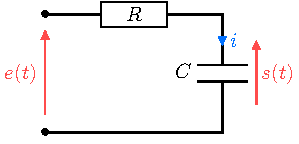
\includegraphics[width=.5\linewidth, draft=true]{filtre_rc}
		}{
			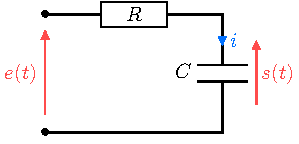
\includegraphics[width=.5\linewidth]{filtre_rc}
		}
		\vspace{-15pt}
		\captionof{figure}{RC sur C.}
	\end{center}
\end{minipage}

\subsubsection{Prévision comportement}
On peut détecter dès cette écriture la nature du filtre en prévoyant son
comportement à hautes et basses fréquences, grâce aux comportements limites des
impédances utilisées~:
\smallbreak
\begin{isd}[sidebyside align=top]
	\tcbsubtitle{\fatbox{Basses fréquences}}
	\noindent
	\begin{minipage}[]{\linewidth}
		\centering
		\sswitch{
			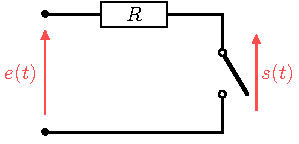
\includegraphics[width=\linewidth, draft=true]{filtre_rc-bf}
		}{
			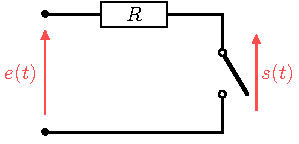
\includegraphics[width=\linewidth]{filtre_rc-bf}
		}
		\vspace{-15pt}
		\captionof{figure}{RC sur C en BF}
	\end{minipage}
	On en déduit~:
	\psw{
		\begin{gather*}
			\text{Circuit ouvert} \Ra i(t) = 0 \Lra \boxed{s(t) = e(t)}
			\\\Ra
			H(0) = 1
			\Lra
			G(0) = 0
			\\\qet
			\Delta\f_{s/e}(0) = 0
		\end{gather*}
	}
	\vspace{-15pt}
	\tcblower
	\tcbsubtitle{\fatbox{Hautes fréquences}}
	\begin{minipage}[]{\linewidth}
		\centering
		\sswitch{
			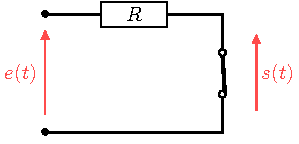
\includegraphics[width=\linewidth, draft=true]{filtre_rc-hf}
		}{
			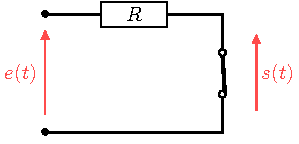
\includegraphics[width=\linewidth]{filtre_rc-hf}
		}
		\vspace{-15pt}
		\captionof{figure}{RC sur C en HF}
	\end{minipage}
	On en déduit~:
	\psw{
		\begin{gather*}
			\text{Tension d'un fil} \Ra \boxed{s(t) = 0}
			\\\Ra
			H(x) \opto{}{\w\to\infty} 0
			\Lra
			G(x) \opto{}{\w\to\infty} -\infty
		\end{gather*}
	}
	\vspace{-15pt}
\end{isd}

\subsubsection{Fonction de transfert, généralisation}
On a trouvé la fonction de transfert plus tôt. On généralise~:
\begin{tcb*}(ror){Généralisation passe-bas ordre 1}
	La forme canonique d'un filtre passe-bas du premier ordre est
	\psw{
		\[
			\boxed{\Hu(x) = \frac{H_0}{1+\jx}}
			\qav
			x = \frac{\w}{\w_c}
			\qet
			H_0 = \cte
		\]
	}
	\vspace{-15pt}
\end{tcb*}

\subsubsection{Diagramme de \textsc{Bode}}
On rappelle les diagrammes de \textsc{Bode}, avec~:
\begin{table}[htbp!]
	\centering
	\caption{Étude RC sur C.}
	\begin{tabularx}{.7\linewidth}{cYYY}
		\toprule
		 &
		$\forall x$
		 &
		$x\to 0$
		 &
		$x\to\infty$
		\\
		\addlinespace[0.5em]
		\cmidrule(lr){2-4}
		$\DS\Hu = \frac{\Su}{\Eu}$
		 &
		\psw{$\DS \frac{1}{1+\jx}$}
		 &
		\psw{$1$}
		 &
		\psw{$\DS \frac{1}{\jx}$}
		\\
		\addlinespace[0.5em]
		$\DS G\ind{dB} = 20 \log \abs{\Hu}$
		 &
		\psw{$\DS -10 \log (1+x^{2})$}
		 &
		\psw{$0$}
		 &
		\psw{$-20 \log (x)$}
		\\
		\addlinespace[0.5em]
		$\DS\Delta\f_{s/e} = \arg*{\Hu}$
		 &
		\psw{$-\arctan(x)$}
		 &
		\psw{$0$}
		 &
		\psw{$\DS-\frac{\pi}{2}$}
		\\
		\bottomrule
	\end{tabularx}
	\label{tab:rcc}
\end{table}
\begin{figure}[htbp!]
	\centering
	\subcaptionbox{Gain\label{fig:rccbodegain}}[.48\linewidth]
	{\sswitch{
			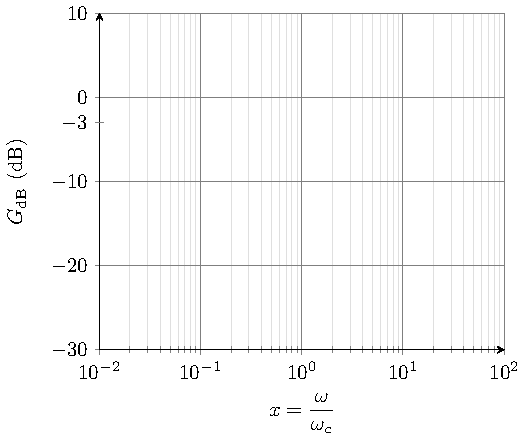
\includegraphics[width=\linewidth]{RCC_bode-gain_plain}
		}{
			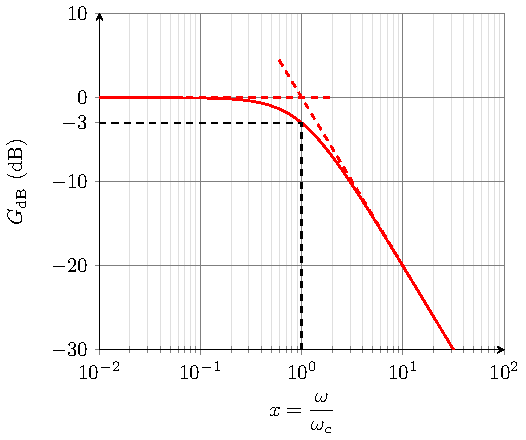
\includegraphics[width=\linewidth]{RCC_bode-gain}
		}
		\vspace{-15pt}
	}%
	\subcaptionbox{Phase\label{fig:rccbodephase}}[.48\linewidth]
	{\sswitch{
			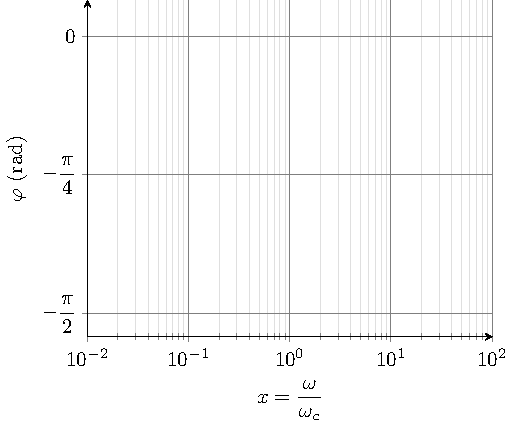
\includegraphics[width=\linewidth]{RCC_bode-phase_plain}
		}{
			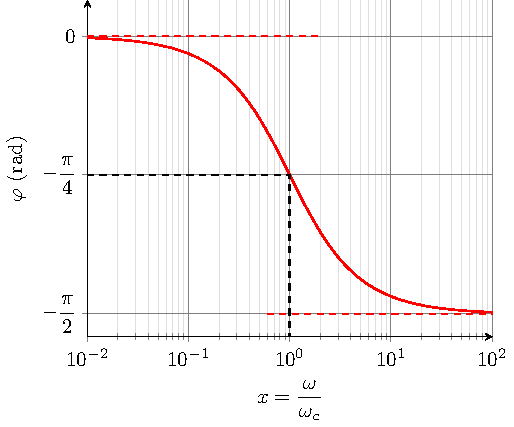
\includegraphics[width=\linewidth]{RCC_bode-phase}
		}
		\vspace{-15pt}
	}%
	\caption{Diagramme de \textsc{Bode} du filtre RC sur C.}
	\label{fig:rccbode}
\end{figure}

\subsubsection{Comportement intégrateur à HF}
En hautes fréquences, la fonction de transfert est celle d'un intégrateur~:
\psw{
	\[
		\Hu(\w) \opto{}{\w\to\infty} \frac{\w_c}{\jw}
		\Lra
		\boxed{\Su \opto{}{\w\to\infty} \frac{\w_c}{\jw}\Eu}
	\]
}
Par exemple, sur un signal créneau, on obtient la figure suivante~:
\begin{figure}[htbp]
	\centering
	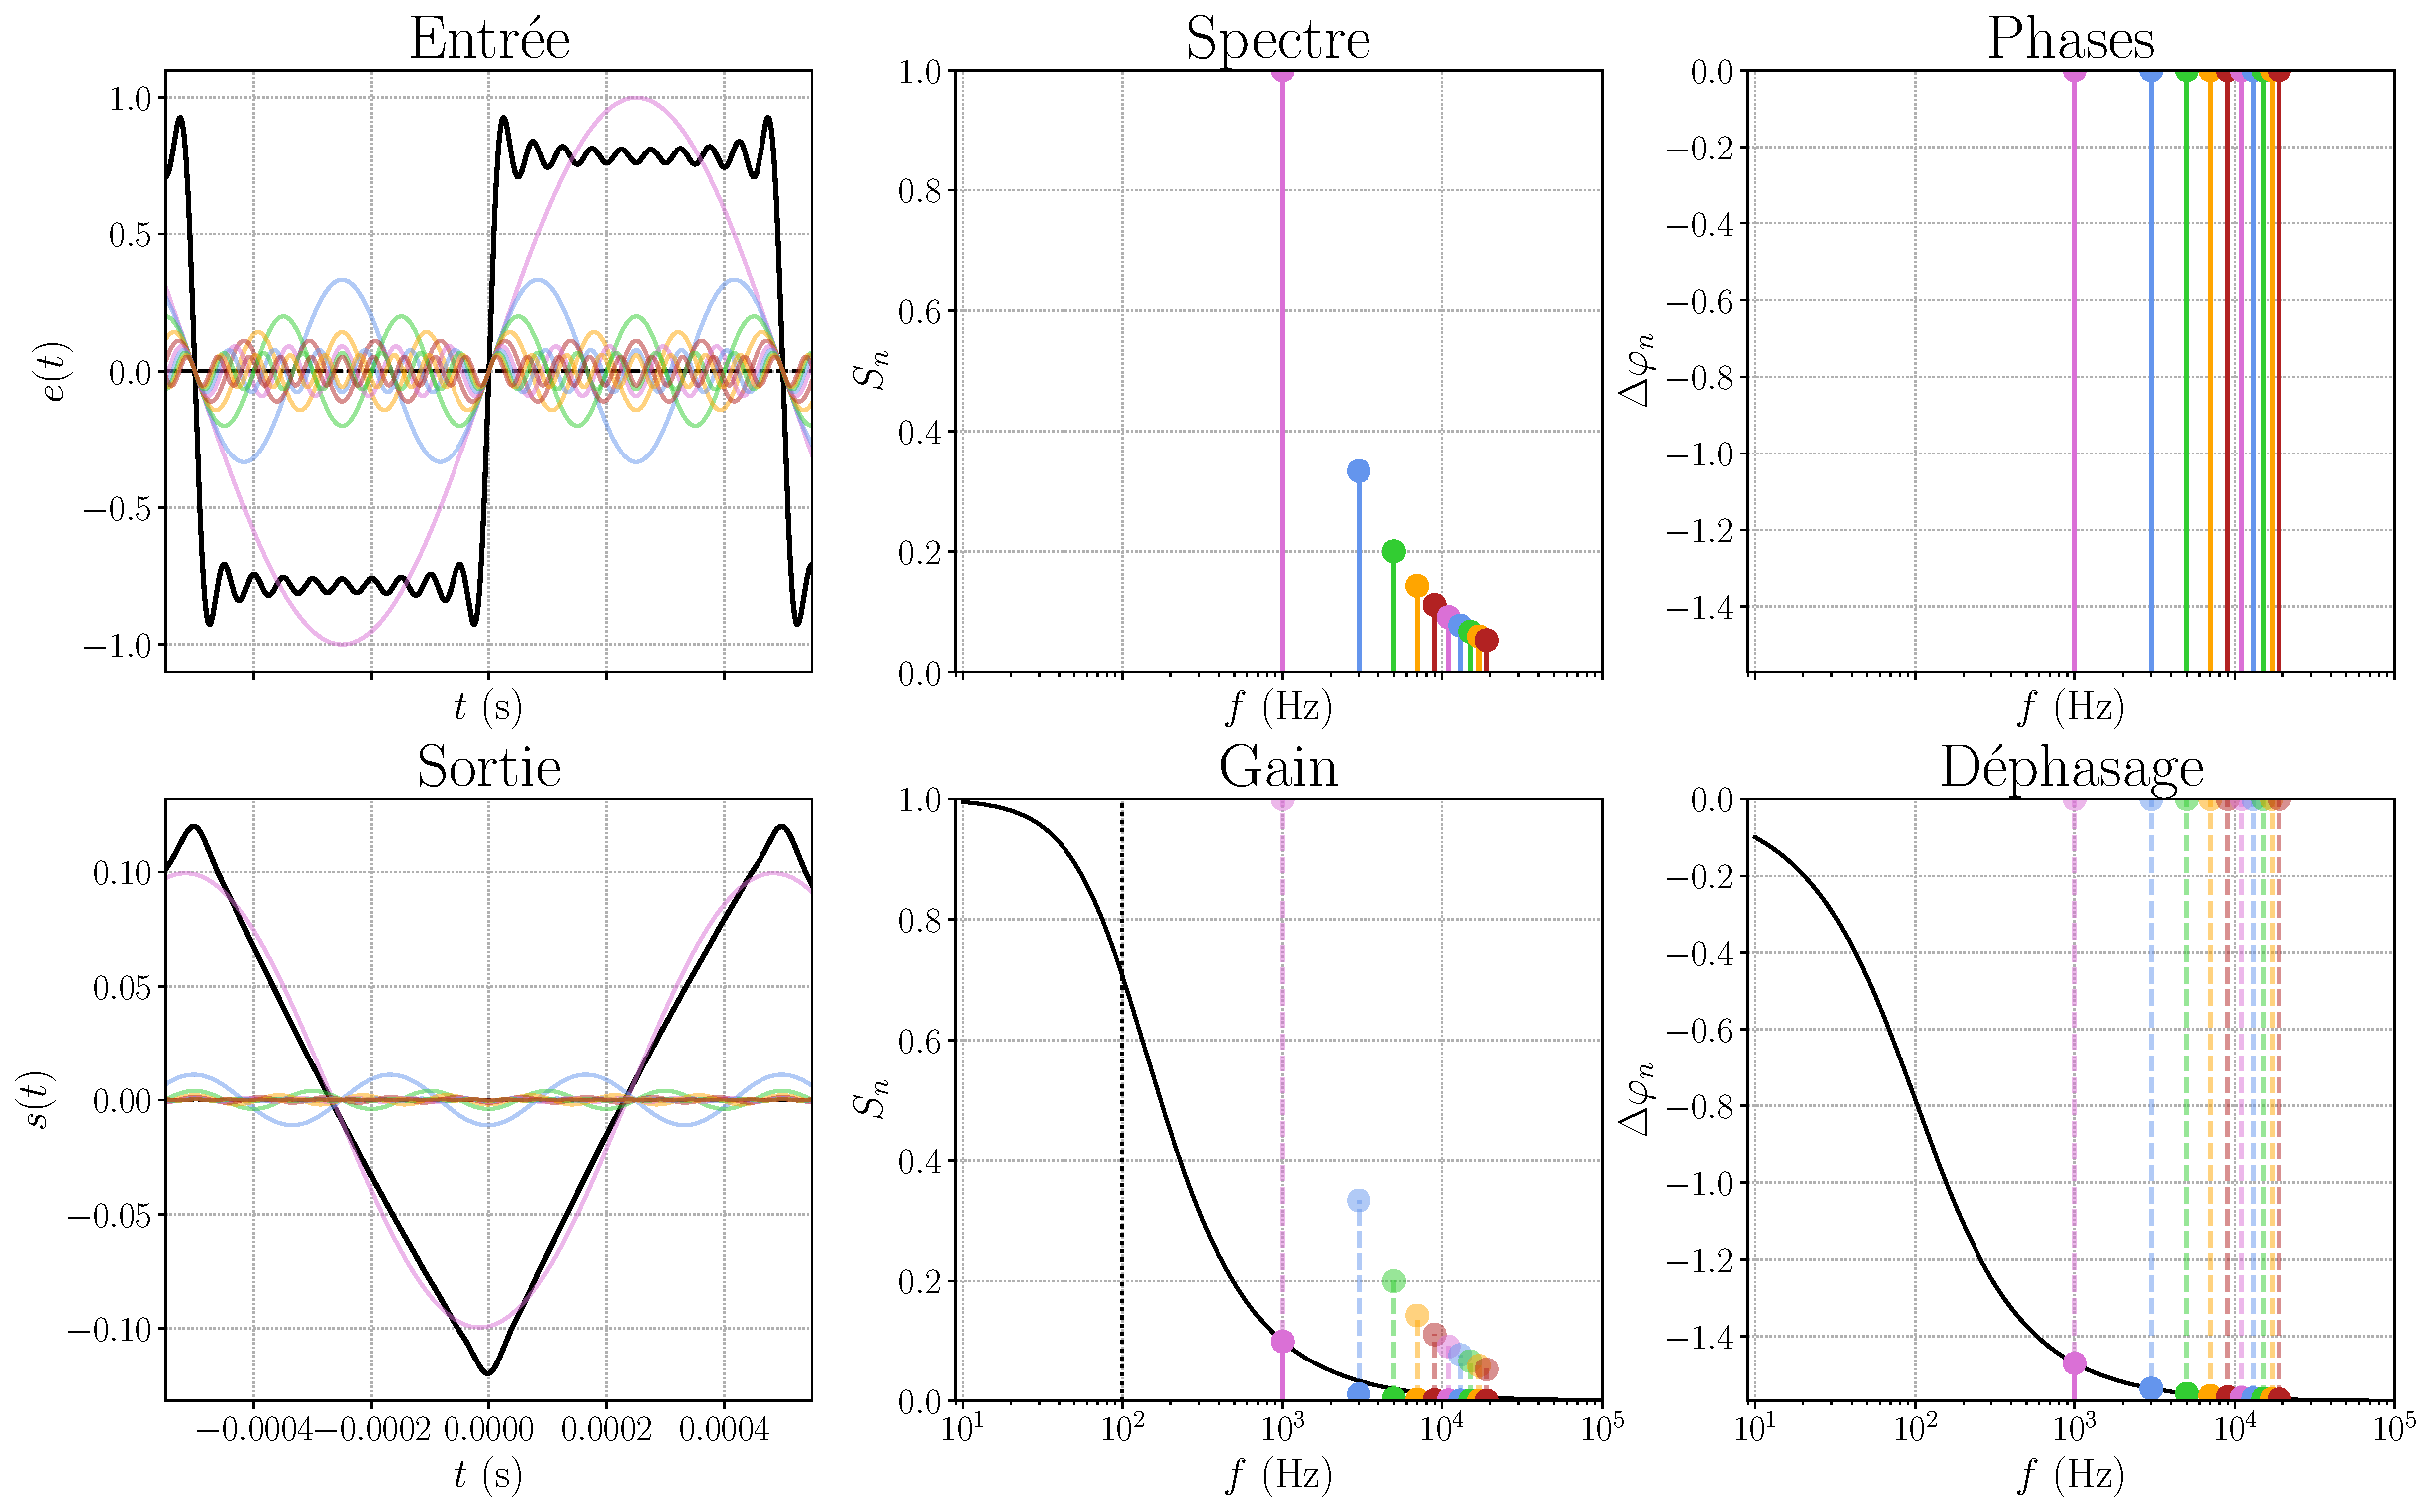
\includegraphics[width=.95\linewidth]{fft_creneau_bth-fe=1000-fc=100}
	\caption{Filtrage d'un signal créneau de $f_e = \SI{1}{kHz}$ par un passe-bas
		de $f_c = \SI{100}{Hz}$.}
	\label{fig:creneauPB}
\end{figure}

\subsection{RC sur R~: passe-haut}
\subsubsection{Schéma}
\smallbreak
\noindent
\begin{minipage}{\linewidth}
	\begin{center}
		\sswitch{
			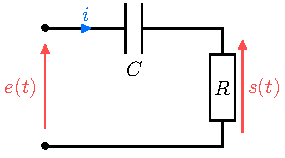
\includegraphics[width=.5\linewidth, draft=true]{filtre_rcr}
		}{
			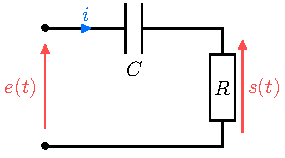
\includegraphics[width=.5\linewidth]{filtre_rcr}
		}
		\vspace{-15pt}
		\captionof{figure}{RC sur R.}
	\end{center}
\end{minipage}

\subsubsection{Prévision comportement}
On peut détecter dès cette écriture la nature du filtre en prévoyant son
comportement à hautes et basses fréquences, grâce aux comportements limites des
impédances utilisées~:
\smallbreak
\begin{isd}[sidebyside align=top]
	\tcbsubtitle{\fatbox{Basses fréquences}}
	\noindent
	\begin{minipage}[]{\linewidth}
		\centering
		\sswitch{
			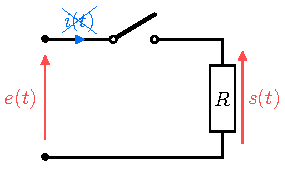
\includegraphics[width=\linewidth, draft=true]{filtre_rcr-bf}
		}{
			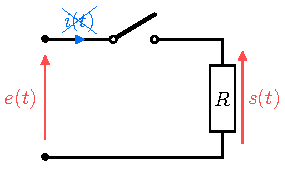
\includegraphics[width=\linewidth]{filtre_rcr-bf}
		}
		\vspace{-15pt}
		\captionof{figure}{RC sur R en BF}
	\end{minipage}
	On en déduit~:
	\psw{
		\begin{gather*}
			\text{Circuit ouvert} \Ra i(t) = 0 \Ra \boxed{s(t) = 0}
			\\\Ra
			H(x) \opto{}{\w\to\infty} 0
			\Lra
			G(x) \opto{}{\w\to\infty} -\infty
		\end{gather*}
	}
	\vspace{-15pt}
	\tcblower
	\tcbsubtitle{\fatbox{Hautes fréquences}}
	\begin{minipage}[]{\linewidth}
		\centering
		\sswitch{
			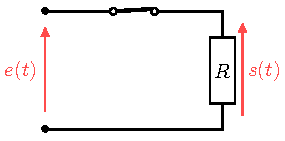
\includegraphics[width=\linewidth, draft=true]{filtre_rcr-hf}
		}{
			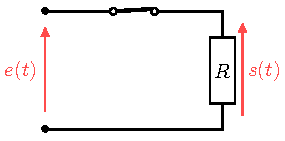
\includegraphics[width=\linewidth]{filtre_rcr-hf}
		}
		\vspace{-15pt}
		\captionof{figure}{RC sur R en HF}
	\end{minipage}
	On en déduit~:
	\psw{
		\begin{gather*}
			\text{LdM} \Ra \boxed{s(t) = e(t)}
			\\\Ra
			H(0) = 1
			\Lra
			G(0) = 0
			\\\qet
			\Delta\f_{s/e}(0) = 0
		\end{gather*}
	}
	\vspace{-15pt}
\end{isd}
C'est donc bien un \textbf{passe-haut}.

\subsubsection{Fonction de transfert, généralisation}
Pour trouver la fonction de transfert, on transforme le circuit en complexes et
on applique un pont diviseur de tension~:
\smallbreak
\noindent
\begin{minipage}[c]{.45\linewidth}
	\begin{center}
		\sswitch{
			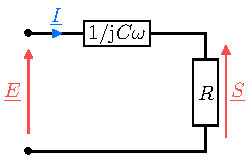
\includegraphics[width=\linewidth, draft=true]{filtre_rcr-cplx}
		}{
			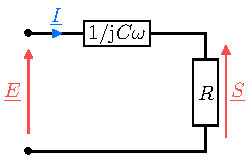
\includegraphics[width=\linewidth]{filtre_rcr-cplx}
		}
		\vspace{-15pt}
		\captionof{figure}{RC en complexes.}
	\end{center}
\end{minipage}
\hfill
\begin{minipage}[c]{.5\linewidth}
	Pont diviseur~:
	\psw{
		\begin{DispWithArrows*}[fleqn, mathindent=-5pt]
			\Su &= \frac{R}{R + 1/\jcw}\Eu
			\CArrow{$\times \frac{\jcw}{\jcw}$}
			\\\Lra
			\Su &= \frac{\jrcw}{1+\jrcw}\Eu
			\Arrow{$\Hu = \Su/\Eu$}
			\\\Lra
			\Aboxed{\Hu &= \frac{\jrcw}{1+\jrcw} =
				\frac{\jj \frac{\w}{\w_c}}{1+\jj \frac{\w}{\w_c}}}
		\end{DispWithArrows*}
		avec $\w_c = \frac{1}{RC}$ la pulsation de coupure.
	}
\end{minipage}
\begin{tcb*}(ror){Généralisation passe-haut ordre 1}
	La forme canonique d'un filtre passe-haut du premier ordre est
	\psw{
		\[
			\boxed{\Hu(x) = H_0\frac{\jx}{1+\jx}}
			\qav
			x = \frac{\w}{\w_c}
			\qet
			H_0 = \cte
		\]
	}
	\vspace{-15pt}
\end{tcb*}

\subsubsection{Diagramme de \textsc{Bode}}
On trace les diagrammes de \textsc{Bode}, avec~:
\begin{table}[htbp!]
	\centering
	\caption{Étude RC sur R.}
	\begin{tabularx}{.7\linewidth}{cYYY}
		\toprule
		 &
		$\forall x$
		 &
		$x\to 0$
		 &
		$x\to\infty$
		\\
		\addlinespace[0.5em]
		\cmidrule(lr){2-4}
		$\DS\Hu = \frac{\Su}{\Eu}$
		 &
		\psw{$\DS \frac{\jx}{1+\jx}$}
		 &
		\psw{$\jx$}
		 &
		\psw{$1$}
		\\
		\addlinespace[0.5em]
		$\DS G\ind{dB} = 20 \log \abs{\Hu}$
		 &
		\psw{$\DS 20 \log \left( \frac{x}{\sqrt{1+x^{2}}} \right)$}
		 &
		\psw{$20 \log x$}
		 &
		\psw{$0$}
		\\
		\addlinespace[0.5em]
		$\DS\Delta\f_{s/e} = \arg*{\Hu}$
		 &
		\psw{$\DS \frac{\pi}{2}-\arctan(x)$}
		 &
		\psw{$\DS \frac{\pi}{2}$}
		 &
		\psw{$0$}
		\\
		\bottomrule
	\end{tabularx}
	\label{tab:rcr}
\end{table}
\begin{figure}[htbp!]
	\centering
	\subcaptionbox{Gain\label{fig:rcrbodegain}}[.48\linewidth]
	{\sswitch{
			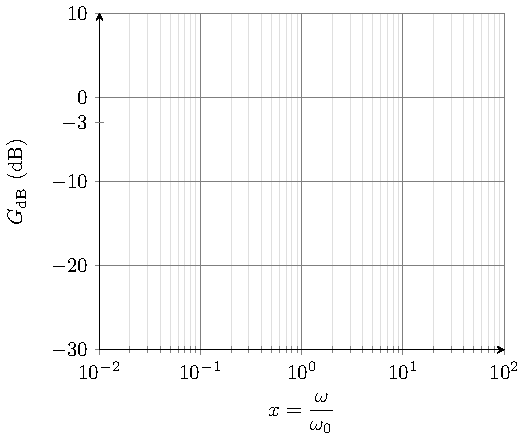
\includegraphics[width=.95\linewidth]{RCR_bode-gain_plain}
		}{
			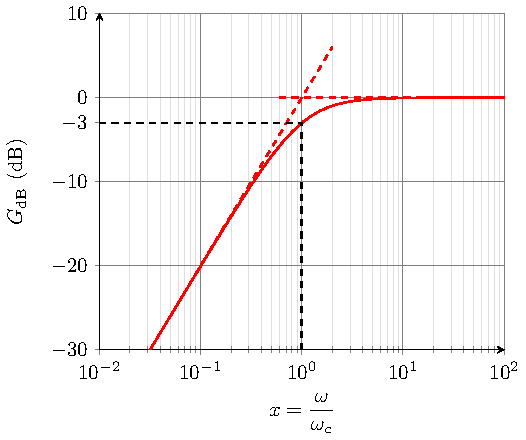
\includegraphics[width=.95\linewidth]{RCR_bode-gain}
		}
		\vspace{-15pt}
	}
	\subcaptionbox{Phase\label{fig:rcrbodephase}}[.48\linewidth]
	{\sswitch{
			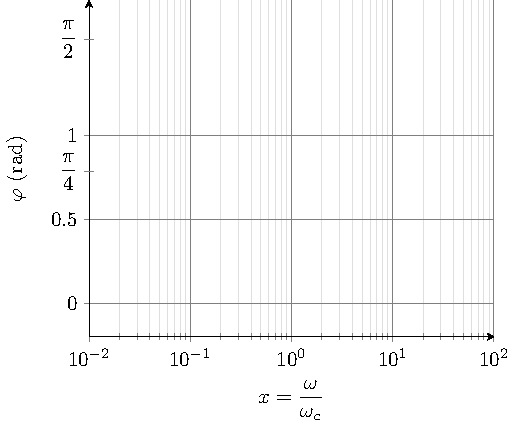
\includegraphics[width=.95\linewidth]{RCR_bode-phase_plain}
		}{
			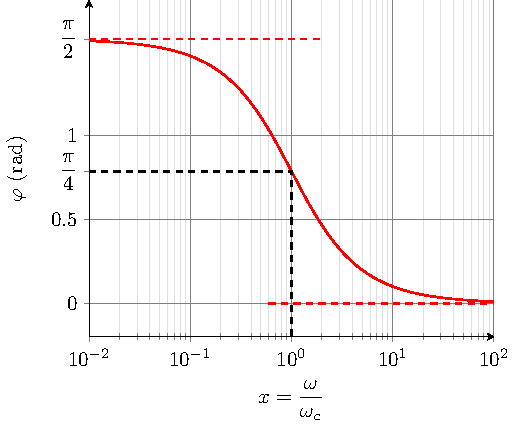
\includegraphics[width=.95\linewidth]{RCR_bode-phase}
		}
		\vspace{-15pt}
	}
	\caption{Diagramme de \textsc{Bode} du filtre RC sur R.}
	\label{fig:rcrbode}
\end{figure}

\subsubsection{Comportement dérivateur à BF}
En basses fréquences, la fonction de transfert est celle d'un dérivateur~:
\psw{
	\[
		\Hu(\w) \opto{}{\w\to\infty} \frac{\jw}{\w_c}
		\Lra
		\boxed{\Su \opto{}{\w\to\infty} \frac{\jw}{\w_c}\Eu}
	\]
}
Par exemple, sur un signal triangle, on obtient la figure suivante~:
\begin{figure}[htbp]
	\centering
	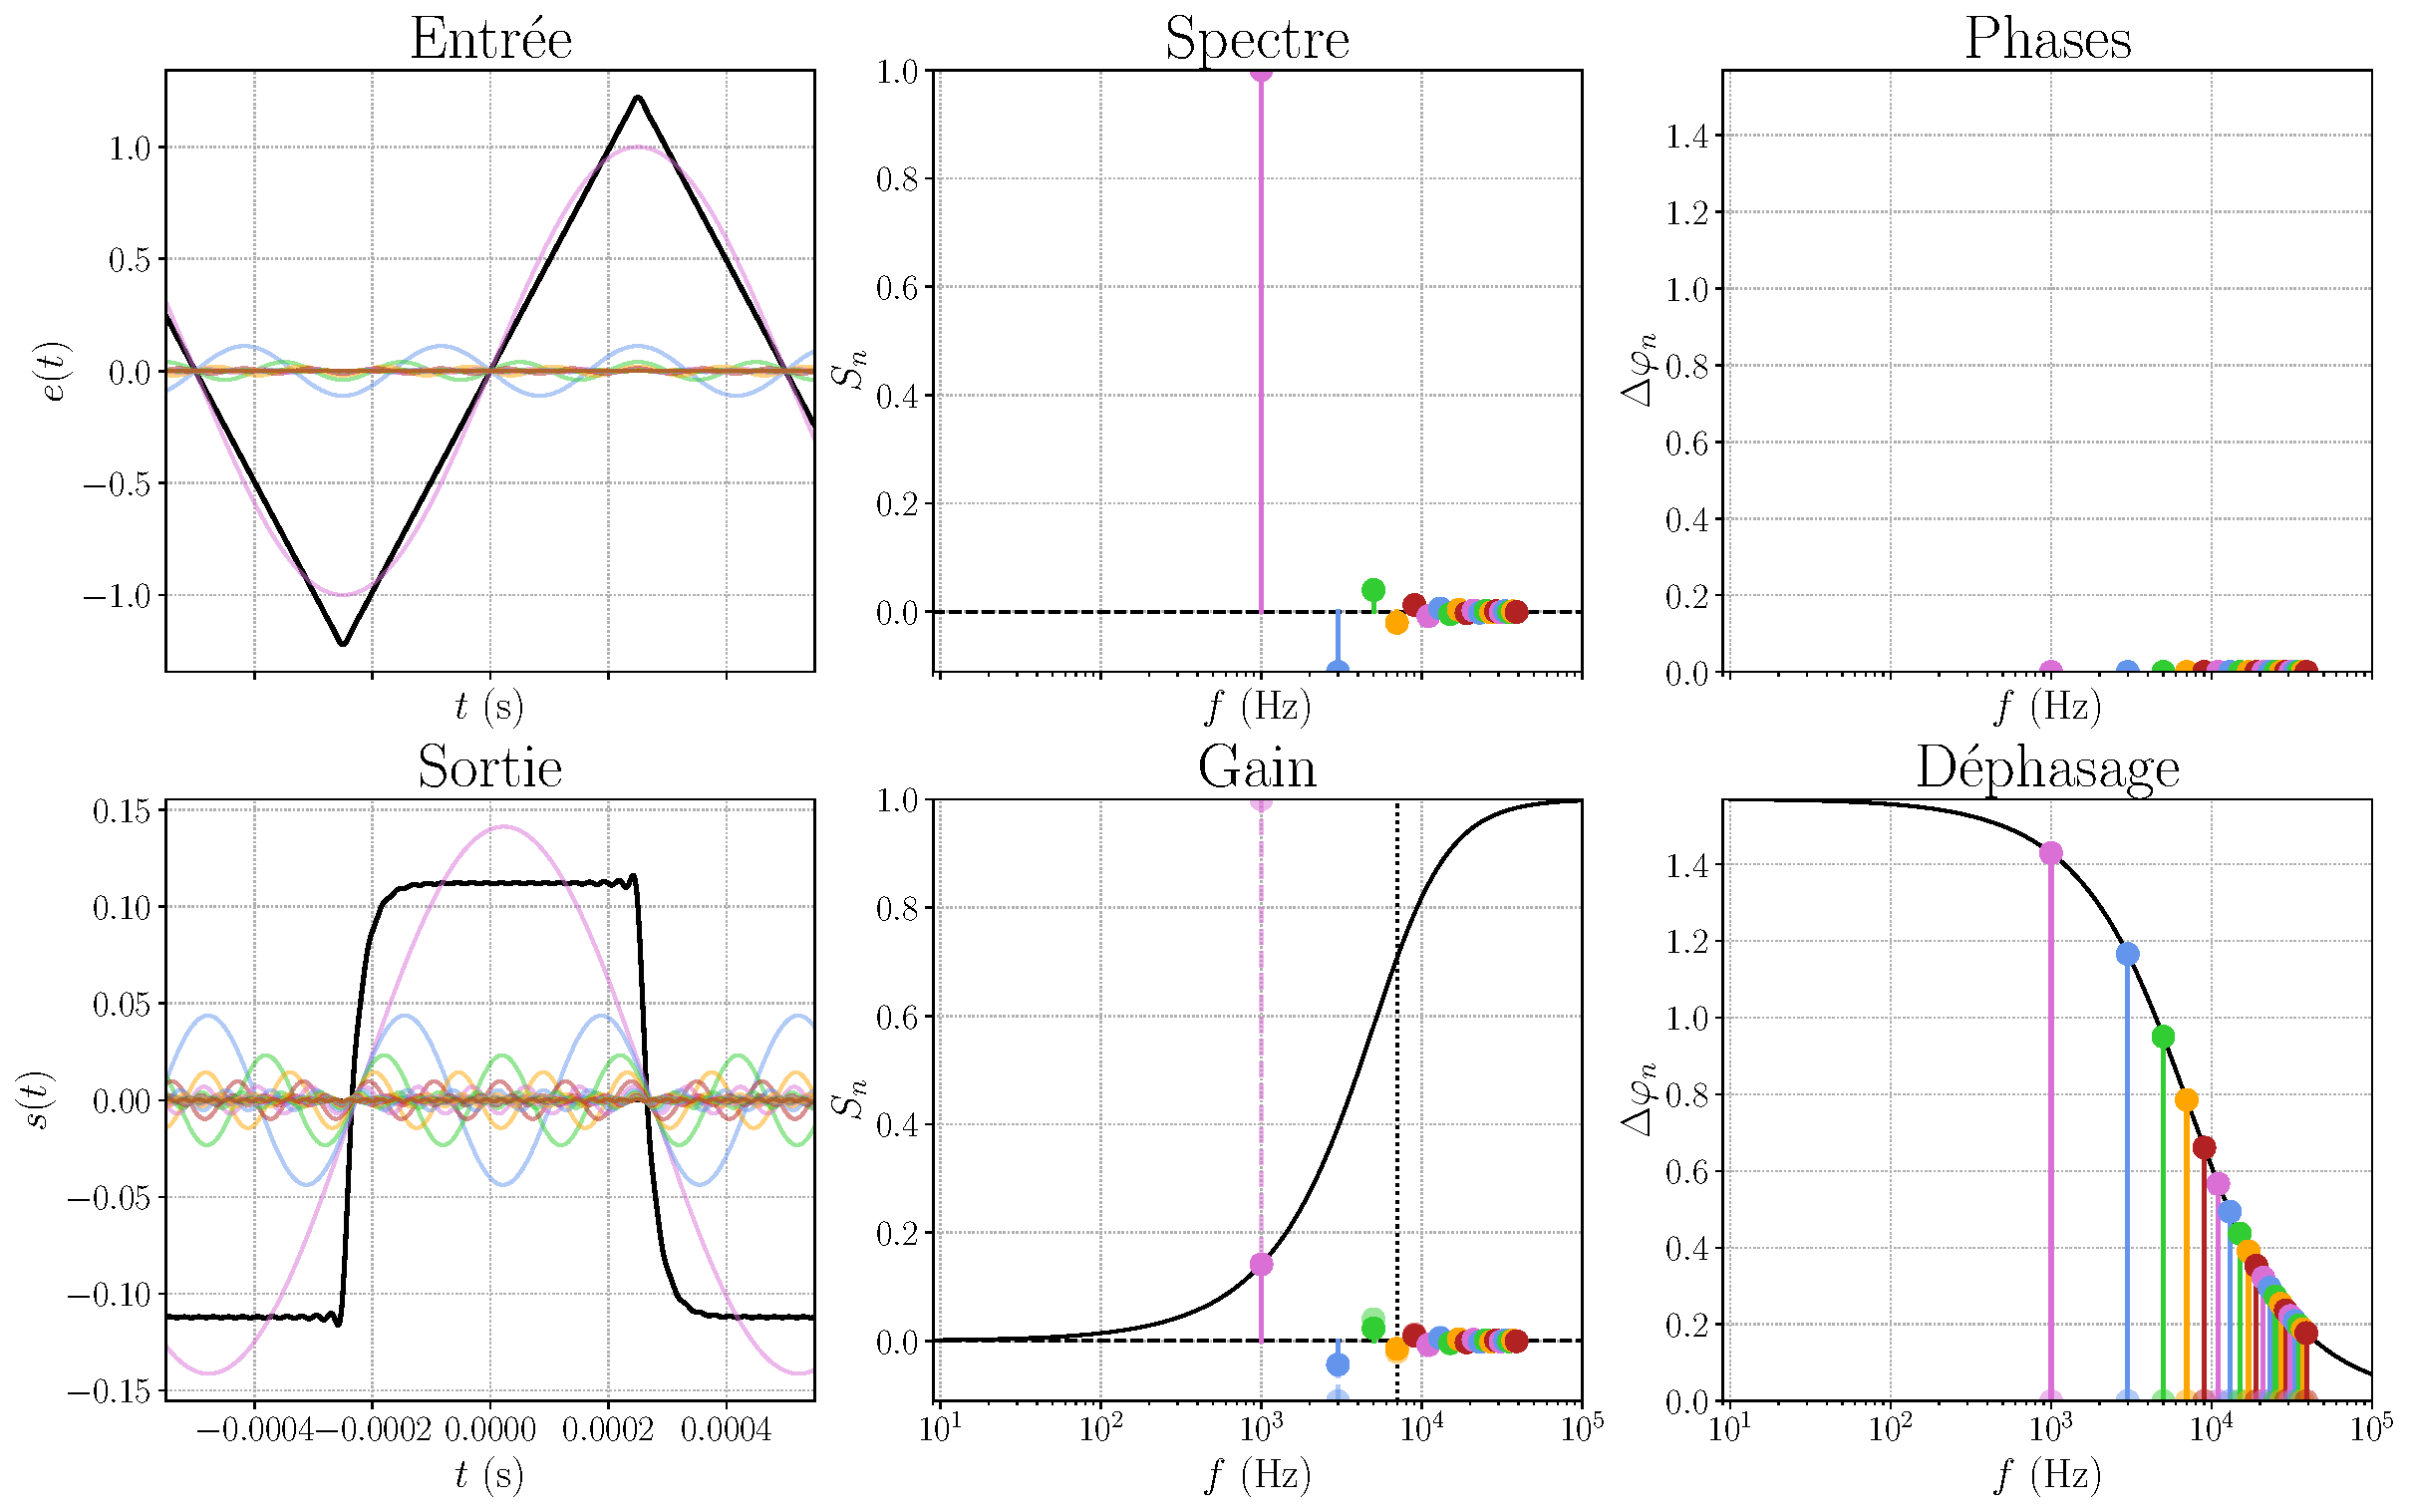
\includegraphics[width=.95\linewidth]{fft_trgl_bth_PH-fe=1000-fc=7000}
	\caption{Filtrage d'un signal triangle de $f_e = \SI{1}{kHz}$ par un
		passe-haut de $f_c = \SI{7000}{Hz}$.}
	\label{fig:trglPH}
\end{figure}
C'est bien un dérivateur.

\section{Exemples de filtres d'ordre 2}
\subsection{RLC sur C~: passe-bas ordre 2}
\subsubsection{Schéma}
\smallbreak
\noindent
\begin{minipage}{\linewidth}
	\begin{center}
		\sswitch{
			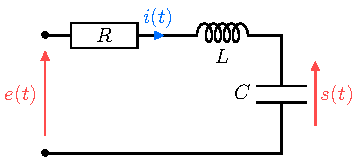
\includegraphics[width=.5\linewidth, draft=true]{filtre_rlc}
		}{
			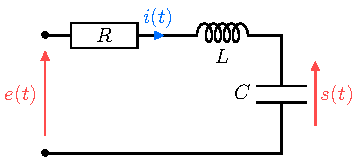
\includegraphics[width=.5\linewidth]{filtre_rlc}
		}
		\vspace{-15pt}
		\captionof{figure}{RLC sur C.}
	\end{center}
\end{minipage}

\subsubsection{Prévision comportement}
On peut détecter dès cette écriture la nature du filtre en prévoyant son
comportement à hautes et basses fréquences, grâce aux comportements limites des
impédances utilisées~:
\smallbreak
\begin{isd}[sidebyside align=top]
	\tcbsubtitle{\fatbox{Basses fréquences}}
	\noindent
	\begin{minipage}[]{\linewidth}
		\centering
		\sswitch{
			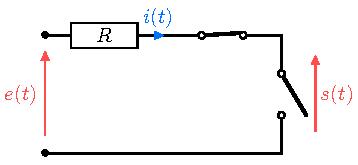
\includegraphics[width=\linewidth, draft=true]{filtre_rlc-bf}
		}{
			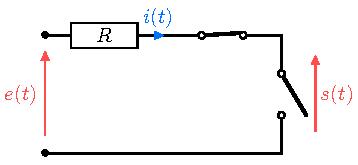
\includegraphics[width=\linewidth]{filtre_rlc-bf}
		}
		\vspace{-15pt}
		\captionof{figure}{RLC sur C en BF}
	\end{minipage}
	On en déduit~:
	\psw{
		\begin{gather*}
			\text{Circuit ouvert} \Ra i(t) = 0 \Lra \boxed{s(t) = e(t)}
			\\\Ra
			H(0) = 1
			\Lra
			G(0) = 0
			\\\qet
			\Delta\f_{s/e}(0) = 0
		\end{gather*}
	}
	\vspace{-15pt}
	\tcblower
	\tcbsubtitle{\fatbox{Hautes fréquences}}
	\begin{minipage}[]{\linewidth}
		\centering
		\sswitch{
			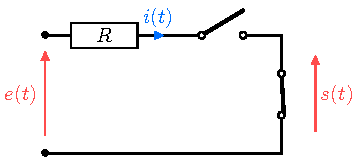
\includegraphics[width=\linewidth, draft=true]{filtre_rlc-hf}
		}{
			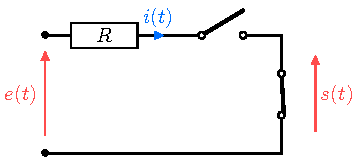
\includegraphics[width=\linewidth]{filtre_rlc-hf}
		}
		\vspace{-15pt}
		\captionof{figure}{RLC sur C en HF}
	\end{minipage}
	On en déduit~:
	\psw{
		\begin{gather*}
			\text{Tension d'un fil} \Ra \boxed{s(t) = 0}
			\\\Ra
			H(x) \opto{}{\w\to\infty} 0
			\Lra
			G(x) \opto{}{\w\to\infty} -\infty
		\end{gather*}
	}
	\vspace{-15pt}
\end{isd}
C'est donc bien un \textbf{passe-bas}.

\subsubsection{Fonction de transfert, généralisation}
Pour trouver la fonction de transfert, on transforme le circuit en complexes et
on applique un pont diviseur de tension~:
\smallbreak
\noindent
\begin{minipage}[c]{.45\linewidth}
	\begin{center}
		\sswitch{
			\includegraphics[width=\linewidth, draft=true]{filtre_rlc-cplx}
		}{
			\includegraphics[width=\linewidth]{filtre_rlc-cplx}
		}
		\vspace{-15pt}
		\captionof{figure}{RLC en complexes.}
	\end{center}
\end{minipage}
\hfill
\begin{minipage}[c]{.5\linewidth}
	Pont diviseur~:
	\psw{
		\begin{DispWithArrows*}[fleqn, mathindent=-5pt]
			\Su &= \frac{1/\jcw}{R + \jlw + 1/\jcw}\Eu
			\CArrow{$\times \frac{\jcw}{\jcw}$}
			\\\Lra
			\Su &= \frac{1}{1 + \jrcw - LCw^{2}}\Eu
			\Arrow{$\Hu = \Su/\Eu$}
			\\\Lra
			\Aboxed{\Hu &=
				\frac{1}{1 - \left(\frac{\w}{\w_0}\right)^{2}+\jj \frac{\w}{Q\w_0}}}
		\end{DispWithArrows*}
		avec $\w_0 = \frac{1}{\sqrt{LC}}$ la pulsation de coupure et $Q =
			\frac{1}{R}\sqrt{\frac{L}{C}}$ le facteur de qualité.
	}
\end{minipage}
\begin{tcb*}(ror){Généralisation passe-bas ordre 2}
	La forme canonique d'un filtre passe-bas du second ordre est
	\psw{
	\[
		\boxed{\Hu(x) = \frac{H_0}{1-x^{2} + \jj \frac{x}{Q}}}
		\qav
		x = \frac{\w}{\w_0}
		\qet
		H_0 = \cte
		\qet
		Q \text{~ facteur de qualité}
	\]
	}
	\vspace{-15pt}
\end{tcb*}

\subsubsection{Diagramme de \textsc{Bode}}
On trace les diagrammes de \textsc{Bode}, avec~:
\smallbreak
\noindent
\begin{minipage}{\linewidth}
	\centering
	\captionof{table}{Étude RLC sur C.}
	\begin{tabularx}{\linewidth}{cYYY}
		\toprule
		 &
		$\forall x$
		 &
		$x\to 0$
		 &
		$x\to\infty$
		\\
		\addlinespace[0.5em]
		\cmidrule(lr){2-4}
		$\DS\Hu = \frac{\Su}{\Eu}$
		 &
		\psw{$\DS \frac{1}{1-x^{2}+\jj \frac{x}{Q}}$}
		 &
		\psw{$1$}
		 &
		\psw{$\DS - \frac{1}{x^{2}}$}
		\\
		\addlinespace[0.5em]
		$\DS G\ind{dB} = 20 \log \abs{\Hu}$
		 &
		\psw{$\DS -10 \log \left(\left(1-x^{2}\right)^{2} + \left( \frac{x}{Q} \right)^{2}\right)$}
		 &
		\psw{$0$}
		 &
		\psw{$-40 \log x$}
		\\
		\addlinespace[0.5em]
		$\DS\tan(\arg*{\Hu})$
		 &
		\psw{$\DS -\frac{x/Q}{1-x^{2}}$}
		 &
		\psw{$0$}
		 &
		\psw{$0$}
		\\
		\addlinespace[0.5em]
		$\DS\Delta\f_{s/e} = \arg*{\Hu}$
		 &
		\psw{$---$}
		 &
		\psw{$0$}
		 &
		\psw{$\DS -\pi$}
		\\
		\bottomrule
	\end{tabularx}
	\label{tab:rlc}
\end{minipage}
\begin{figure}[htbp!]
	\centering
	\subcaptionbox{Gain\label{fig:rlcbodegain}}[.48\linewidth]
	{\sswitch{
			\includegraphics[width=.95\linewidth]{RLCC_bode-gain_plain}
		}{
			\includegraphics[width=.95\linewidth]{RLCC_bode-gain}
		}
		\vspace{-15pt}
	}
	\subcaptionbox{Phase\label{fig:rlcbodephase}}[.48\linewidth]
	{\sswitch{
			\includegraphics[width=.95\linewidth]{RLCC_bode-phase_plain}
		}{
			\includegraphics[width=.95\linewidth]{RLCC_bode-phase}
		}
		\vspace{-15pt}
	}
	\caption{Diagramme de \textsc{Bode} du filtre RLC sur C.}
	\label{fig:rlcbode}
\end{figure}

On observe donc une pente de \textbf{\SI{-40}{dB/décade}} en atténuation à
grandes fréquences~: ce filtre sera meilleur en moyenneur.

\subsection{RLC sur R~: passe-bande}
\subsubsection{Schéma}
\smallbreak
\noindent
\begin{minipage}{\linewidth}
	\begin{center}
		\sswitch{
			\includegraphics[width=.5\linewidth, draft=true]{filtre_rlcr}
		}{
			\includegraphics[width=.5\linewidth]{filtre_rlcr}
		}
		\vspace{-15pt}
		\captionof{figure}{RLC sur R.}
	\end{center}
\end{minipage}

\subsubsection{Prévision comportement}
On peut détecter dès cette écriture la nature du filtre en prévoyant son
comportement à hautes et basses fréquences, grâce aux comportements limites des
impédances utilisées~:
\smallbreak
\begin{isd}[sidebyside align=top]
	\tcbsubtitle{\fatbox{Basses fréquences}}
	\noindent
	\begin{minipage}[]{\linewidth}
		\centering
		\sswitch{
			\includegraphics[width=\linewidth, draft=true]{filtre_rlcr-bf}
		}{
			\includegraphics[width=\linewidth]{filtre_rlcr-bf}
		}
		\vspace{-15pt}
		\captionof{figure}{RLC sur R en BF}
	\end{minipage}
	On en déduit~:
	\psw{
		\begin{gather*}
			\text{Circuit ouvert} \Ra i(t) = 0 \Lra \boxed{s(t) = 0}
			\\\Ra
			H(x) \opto{}{\w\to\infty} 0
			\Lra
			G(x) \opto{}{\w\to\infty} -\infty
		\end{gather*}
	}
	\vspace{-15pt}
	\tcblower
	\tcbsubtitle{\fatbox{Hautes fréquences}}
	\begin{minipage}[]{\linewidth}
		\centering
		\sswitch{
			\includegraphics[width=\linewidth, draft=true]{filtre_rlcr-hf}
		}{
			\includegraphics[width=\linewidth]{filtre_rlcr-hf}
		}
		\vspace{-15pt}
		\captionof{figure}{RLC sur R en HF}
	\end{minipage}
	On en déduit~:
	\psw{
		\begin{gather*}
			\text{Circuit ouvert} \Ra i(t) = 0 \Lra \boxed{s(t) = 0}
			\\\Ra
			H(x) \opto{}{\w\to\infty} 0
			\Lra
			G(x) \opto{}{\w\to\infty} -\infty
		\end{gather*}
	}
	\vspace{-15pt}
\end{isd}
C'est donc bien un \textbf{passe-bande}.

\subsubsection{Fonction de transfert, généralisation}
Pour trouver la fonction de transfert, on transforme le circuit en complexes et
on applique un pont diviseur de tension~:
\smallbreak
\noindent
\begin{minipage}[c]{.45\linewidth}
	\begin{center}
		\sswitch{
			\includegraphics[width=\linewidth, draft=true]{filtre_rlcr-cplx}
		}{
			\includegraphics[width=\linewidth]{filtre_rlcr-cplx}
		}
		\vspace{-15pt}
		\captionof{figure}{RLC en complexes.}
	\end{center}
\end{minipage}
\hfill
\begin{minipage}[c]{.5\linewidth}
	Pont diviseur~:
	\psw{
		\begin{DispWithArrows*}[fleqn, mathindent=-5pt]
			\Su &= \frac{R}{R + \jlw + 1/\jcw}\Eu
			\CArrow{$\times \frac{1/R}{1/R}$}
			\\\Lra
			\Su &= \frac{1}{1 + \jj \frac{L}{R}\w - \jj \frac{1}{RC\w}}\Eu
			\Arrow{$\Hu = \Su/\Eu$}
			\\\Lra
			\Aboxed{\Hu &=
				\frac{1}{1 + \jj Q \left( x - \frac{1}{x} \right)}}
		\end{DispWithArrows*}
		avec $\w_0 = \frac{1}{\sqrt{LC}}$ la pulsation de coupure et $Q =
			\frac{1}{R}\sqrt{\frac{L}{C}}$ le facteur de qualité.
	}
\end{minipage}
\begin{tcb*}(ror){Généralisation passe-bande ordre 2}
	La forme canonique d'un filtre passe-bande du second ordre est
	\psw{
		\[
			\boxed{\Hu(x) = \frac{H_0}{1 + \jj Q \left( x - \frac{1}{x} \right)}}
			\qav
			x = \frac{\w}{\w_0}
			\qet
			H_0 = \cte
			\qet
			Q \text{~ facteur de qualité}
		\]
	}
	\vspace{-15pt}
\end{tcb*}
\subsubsection{Diagramme de \textsc{Bode}}
On trace les diagrammes de \textsc{Bode}, avec les informations du
Tableau~\ref{tab:rlcr}.
\begin{table}[htbp!]
	\centering
	\caption{Étude RLC sur R.}
	\begin{tabularx}{\linewidth}{cYYY}
		\toprule
		 &
		$\forall x$
		 &
		$x\to 0$
		 &
		$x\to\infty$
		\\
		\addlinespace[0.5em]
		\cmidrule(lr){2-4}
		$\DS\Hu = \frac{\Su}{\Eu}$
		 &
		\psw{$\DS \frac{1}{1+ \jj Q \left( x - \frac{1}{x} \right)}$}
		 &
		\psw{$\DS \jj \frac{x}{Q}$}
		 &
		\psw{$\DS -\jj \frac{1}{xQ}$}
		\\
		\addlinespace[0.5em]
		$\DS G\ind{dB} = 20 \log \abs{\Hu}$
		 &
		\psw{$\DS -10 \log (1+Q^{2}\left( x - \frac{1}{x} \right)^{2})$}
		 &
		\psw{$\DS 20 \log \left( \frac{x}{Q} \right)$}
		 &
		\psw{$\DS -20 \log (Qx)$}
		\\
		\addlinespace[0.5em]
		$\DS\Delta\f_{s/e} = \arg*{\Hu}$
		 &
		\psw{$-\arctan(Q \left( x - \frac{1}{x} \right))$}
		 &
		\psw{$\DS + \frac{\pi}{2}$}
		 &
		\psw{$\DS -\frac{\pi}{2}$}
		\\
		\bottomrule
	\end{tabularx}
	\label{tab:rlcr}
\end{table}
\begin{figure}[htbp!]
	\centering
	\subcaptionbox{Gain\label{fig:rlcrbodegain}}[.48\linewidth]
	{\sswitch{
			\includegraphics[width=.95\linewidth]{RLCR_bode-gain_plain}
		}{
			\includegraphics[width=.95\linewidth]{RLCR_bode-gain}
		}
		\vspace{-15pt}
	}
	\subcaptionbox{Phase\label{fig:rlcrbodephase}}[.48\linewidth]
	{\sswitch{
			\includegraphics[width=.95\linewidth]{RLCR_bode-phase_plain}
		}{
			\includegraphics[width=.95\linewidth]{RLCR_bode-phase}
		}
		\vspace{-15pt}
	}
	\caption{Diagramme de \textsc{Bode} du filtre RLC sur R.}
	\label{fig:rlcrbode}
\end{figure}
On observe, sur la Figure~\ref{fig:rlcrbodegain}, une pente de
\textbf{\SI{20}{dB/décade}} en atténuation à basses fréquences, et
\textbf{\SI{-20}{dB/décade}} à hautes fréquences~: ce filtre permettra d'isoler
des fréquences dans un signal. Par exemple, sur un signal créneau, on obtient la
Figure~\ref{fig:creneauPBD}.
\begin{figure}[htbp]
	\centering
	\includegraphics[width=.95\linewidth]{fft_creneau_bth_bande-fe=1000-fc=5000}
	\caption{Filtrage d'un signal créneau de $f_e = \SI{1}{kHz}$ par un
		passe-bande de $f_c = \SI{5000}{Hz}$.}
	\label{fig:creneauPBD}
\end{figure}

\section{Résumé}
\begin{tcb*}(tool){Étude d'un filtre}
	\begin{enumerate}
		\item On fait l'étude à basses et hautes fréquences~;
		\item On écrit le circuit avec les amplitudes complexes et les impédances des
		      composants~;
		\item On fait un pont diviseur~;
		\item On calcule l'amplitude complexe puis on en déduit la fonction de
		      transfert~;
		\item On calcule le gain en décibels et la phase~;
		\item On fait l'étude asymptotique~;
		\item On trace le diagramme de \textsc{Bode}.
	\end{enumerate}
	Ensuite, pour connaître le signal de sortie d'un signal d'entrée, on le
	décompose en série de \textsc{Fourier} et on applique la fonction de transfert
	complexe à chacune des composantes pour reconstituer le signal de sortie~:
	\[
		e(t) =
		\left\{
		\begin{array}{ccccc}
			E_0                    & \ra & \fbox{$\Hu(0\jw_e)$} & \ra & S_0
			\\
			+                      &     &                      &     & +
			\\
			E_1\sin(\w_e t + \f_1) & \ra & \fbox{$\Hu(1\jw_e)$} & \ra & S_1\sin(\w_e t + \psi_1)
			\\
			+                      &     &                      &     & +
			\\
			E_2\sin(\w_e t + \f_2) & \ra & \fbox{$\Hu(2\jw_e)$} & \ra & S_2\sin(\w_e t + \psi_2)
			\\
			\vdots                 &     &                      &     & \vdots
			\\
			E_n\sin(\w_e t + \f_n) & \ra & \fbox{$\Hu(n\jw_e)$} & \ra & S_n\sin(\w_e t + \psi_n)
		\end{array}
		\right\} = s(t)
	\]
\end{tcb*}


\section{Filtres en cascade}
On appelle «~mettre en cascade~» le fait d'utiliser la sortie d'un filtre comme
l'entrée d'un nouveau. Par exemple, avec deux RC~:
\begin{figure}[htbp]
	\centering
	\includegraphics[width=.5\linewidth]{filtre_rcrc}
	\caption{RC en cascade}
	\label{fig:rcrc}
\end{figure}
On pourrait s'attendre à ce que la fonction de transfert soit
\[
	\Hu = \Hu_1\Hu_2 = \frac{1}{1+\jj R_1C_1\w} \frac{1}{1+\jj R_2C_2\w}
\]
Cependant, le calcul de la fonction de transfert donne
\[
	\Hu = \frac{1}{1 + \jj R_1C_1\w + \jj R_2C_2\w + \boxed{\jj R_1C_2\w} +
		(\jw)^{2}R_1C_1R_2C_2}
\]
\begin{tcb}[cnt, bld](impo){Filtres en cascades}
	Lorsque l'on place des filtres en cascade, la fonction de transfert totale
	n'est pas le produit des fonctions de transfert de chaque étage.
\end{tcb}

Pour appliquer le pont diviseur de tension sur le premier RC, il faut que le
condensateur $C_1$ et la résistance $R_1$ soient parcourus par le même courant,
que le courant partant dans la deuxième branche soit très faible devant le
courant de la première. Cela revient à ce que l'impédance du condensateur soit
très faible devant celle de l'ensemble $R_2C_2$.

\begin{tcb}[cnt](ror){Filtres en cascades}
	Pour que l'on puisse faire le produit des fonctions de transfert, il faut que
	l'impédance de sortie du premier filtre soit faible devant l'impédance d'entrée
	du second, de sorte à négliger le courant dévié par le second étage.
\end{tcb}

En pratique, on emploie souvent des montages utilisant des amplificateurs
opérationnels qui ont une très grande impédance d'entrée. On peut par exemple
intercaler un montage suiveur entre les deux filtres RC.

\end{document}
